\setchapterstyle{kao}
\setchapterpreamble[u]{\margintoc}


\chapter{The IceCube Neutrino Observatory}
\labch{icecube}

The IceCube Neutrino Observatory~\sidecite[6cm]{2017JInst..12P3012A_Instrumentation_Systems} is a cubic-kilometer, ice-Cherenkov detector located at the geographic South Pole. IceCube utilizes the Antarctic glacial ice as detector medium to observe neutrinos by measuring the Cherenkov light produced from secondary charged particles. It was deployed between 2006 and 2011 and has been taking data since the installation of the first modules. The primary goal of IceCube is the observation of astrophysical neutrinos as a telescope, but it can also be used to study fundamental particle physics properties using the same astrophysical neutrinos, and by measuring atmospheric neutrinos as well as studying cosmic rays.


\section{Detector Components} \labsec{icecube_array}

\begin{figure}[h]
    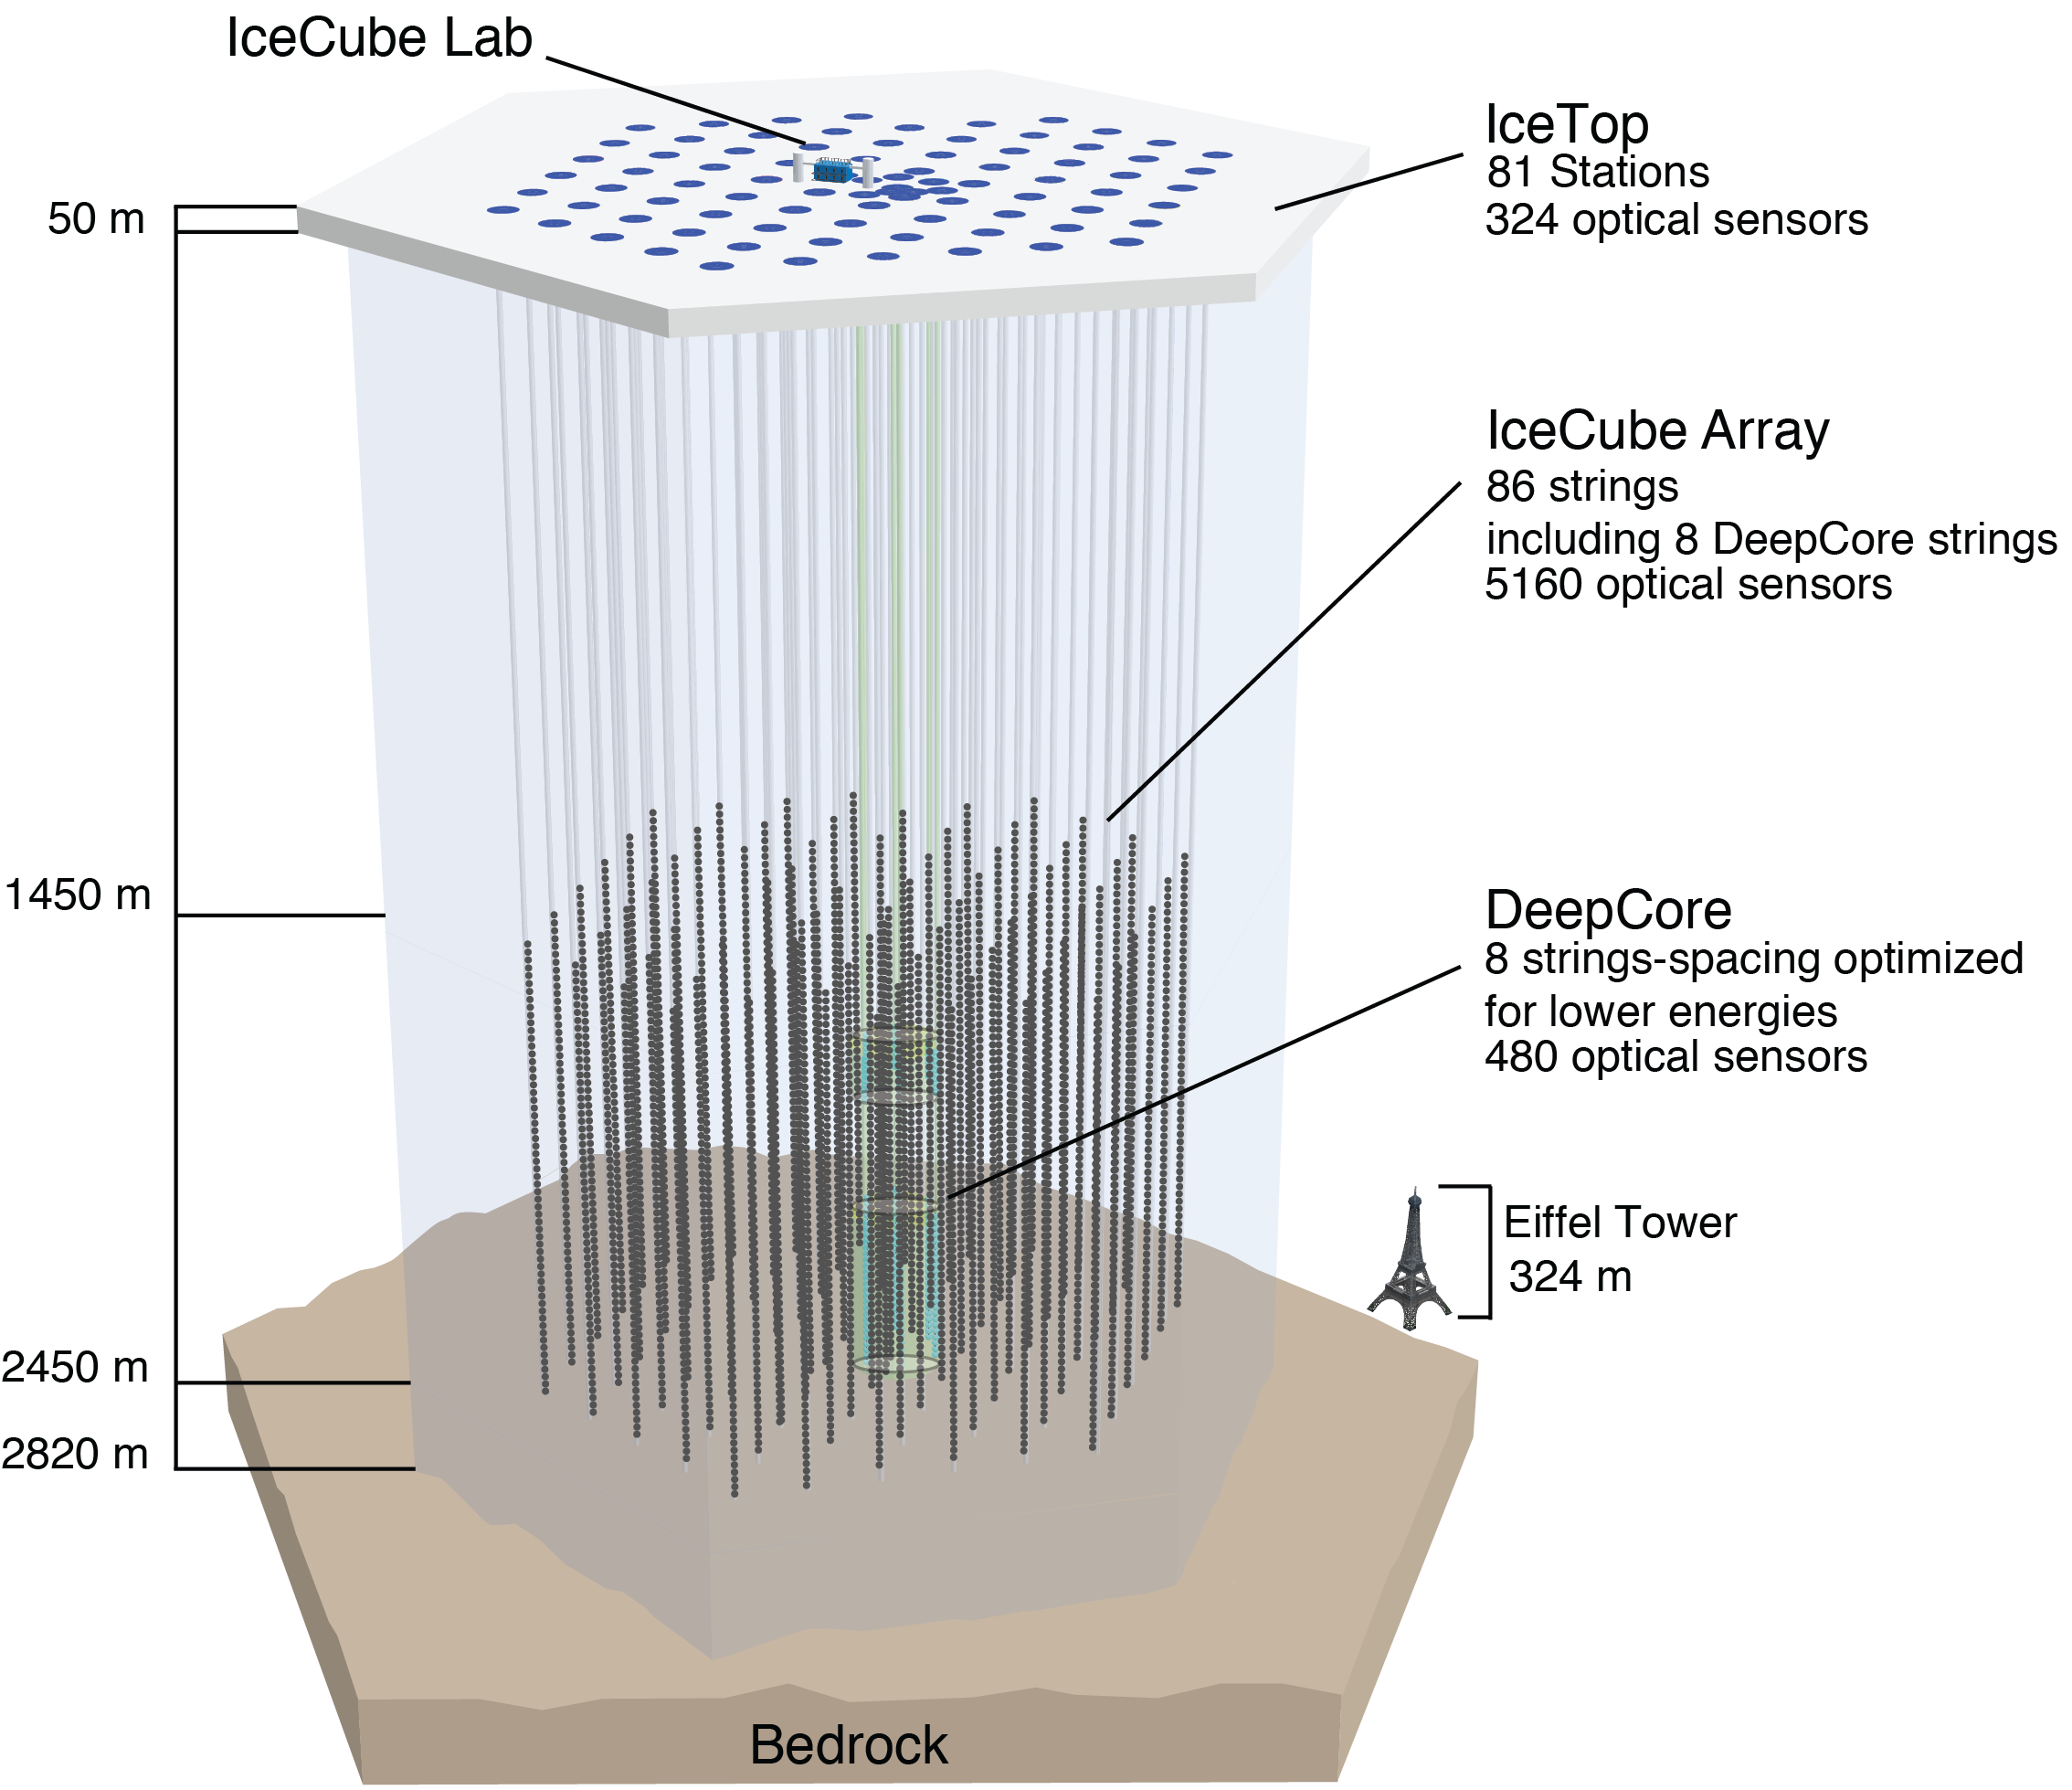
\includegraphics{figures/icecube_deepcore/IceCubeArray_slim.png}
	\caption[IceCube overview]{Overview of the IceCube detector showing the in-ice main- and sub-array IceCube and DeepCore, IceTop, and the IceCube Laboratory. From~\cite{2017JInst..12P3012A_Instrumentation_Systems}.}
    \labfig{icecube_array}
\end{figure}

The full IceCube detector array consists of 86 vertical, in-ice strings and 81 surface stations as shown in \reffig{icecube_array}. The in-ice part is composed of 60 optical modules per string deployed at depths of \SIrange[range-phrase={~-~}]{1450}{2450}{\meter} below the ice, while the surface stations of the cosmic air-shower array, \textit{IceTop}, are ice-filled tanks. The surface stations and the majority of the strings are arranged in a hexagonal grid with the operations building, the \textit{IceCube Laboratory} (ICL), central to the grid on the surface. A top view of the hexagonal arrangement is shown in \reffig{icecube_top_view}. The in-ice array is designed to detect neutrinos in the energy range from \si{\giga\electronvolt} to \si{\peta\electronvolt}.


\subsection{Digital Optical Modules and the Antarctic Ice} \labsec{ice_and_DOMs}

The IceCube detection medium is the Antarctic glacial ice itself, which was formed over \SI{100000}{years} by accumulation of snow that was subsequently compressed by its own weight to form a dense crystal structure~\sidecite{glacial_ice}. As a result of this formation process, the optical properties primarily change with depth. Cherenkov light propagating through the ice is subject to scattering and absorption, which are the two most important ice properties for the detection of neutrinos. Within the detector volume the absorption length ranges from \SIrange[range-phrase={~-~}]{100}{400}{\meter}, while the scattering length lies between \SIrange[range-phrase={~and~}]{20}{100}{\meter}~\sidecite{icecube_ice_paper}. The absorption length is the distance at which the survival probability of the light is reduced to $1/e$ of its original value, while the scattering length is defined as the average distance between scatters. In the antarctic ice, they are correlated, with the absorption length being roughly four times the scattering length~\sidecite{ice_calibration}. The vertical distribution of the inverse absorption length can be seen in \reffig{ic_dc_sidecut}, where one dominant feature is the \textit{dust layer} between \SIrange[range-phrase={~and~}]{2000}{2100}{\meter} depth. This region has a higher concentration of dust particles that were deposited in a period of high volcanic activity, which leads to bad optical properties in form of larger scattering and absorption~\cite{icecube_ice_paper}.


\begin{figure}[h]
    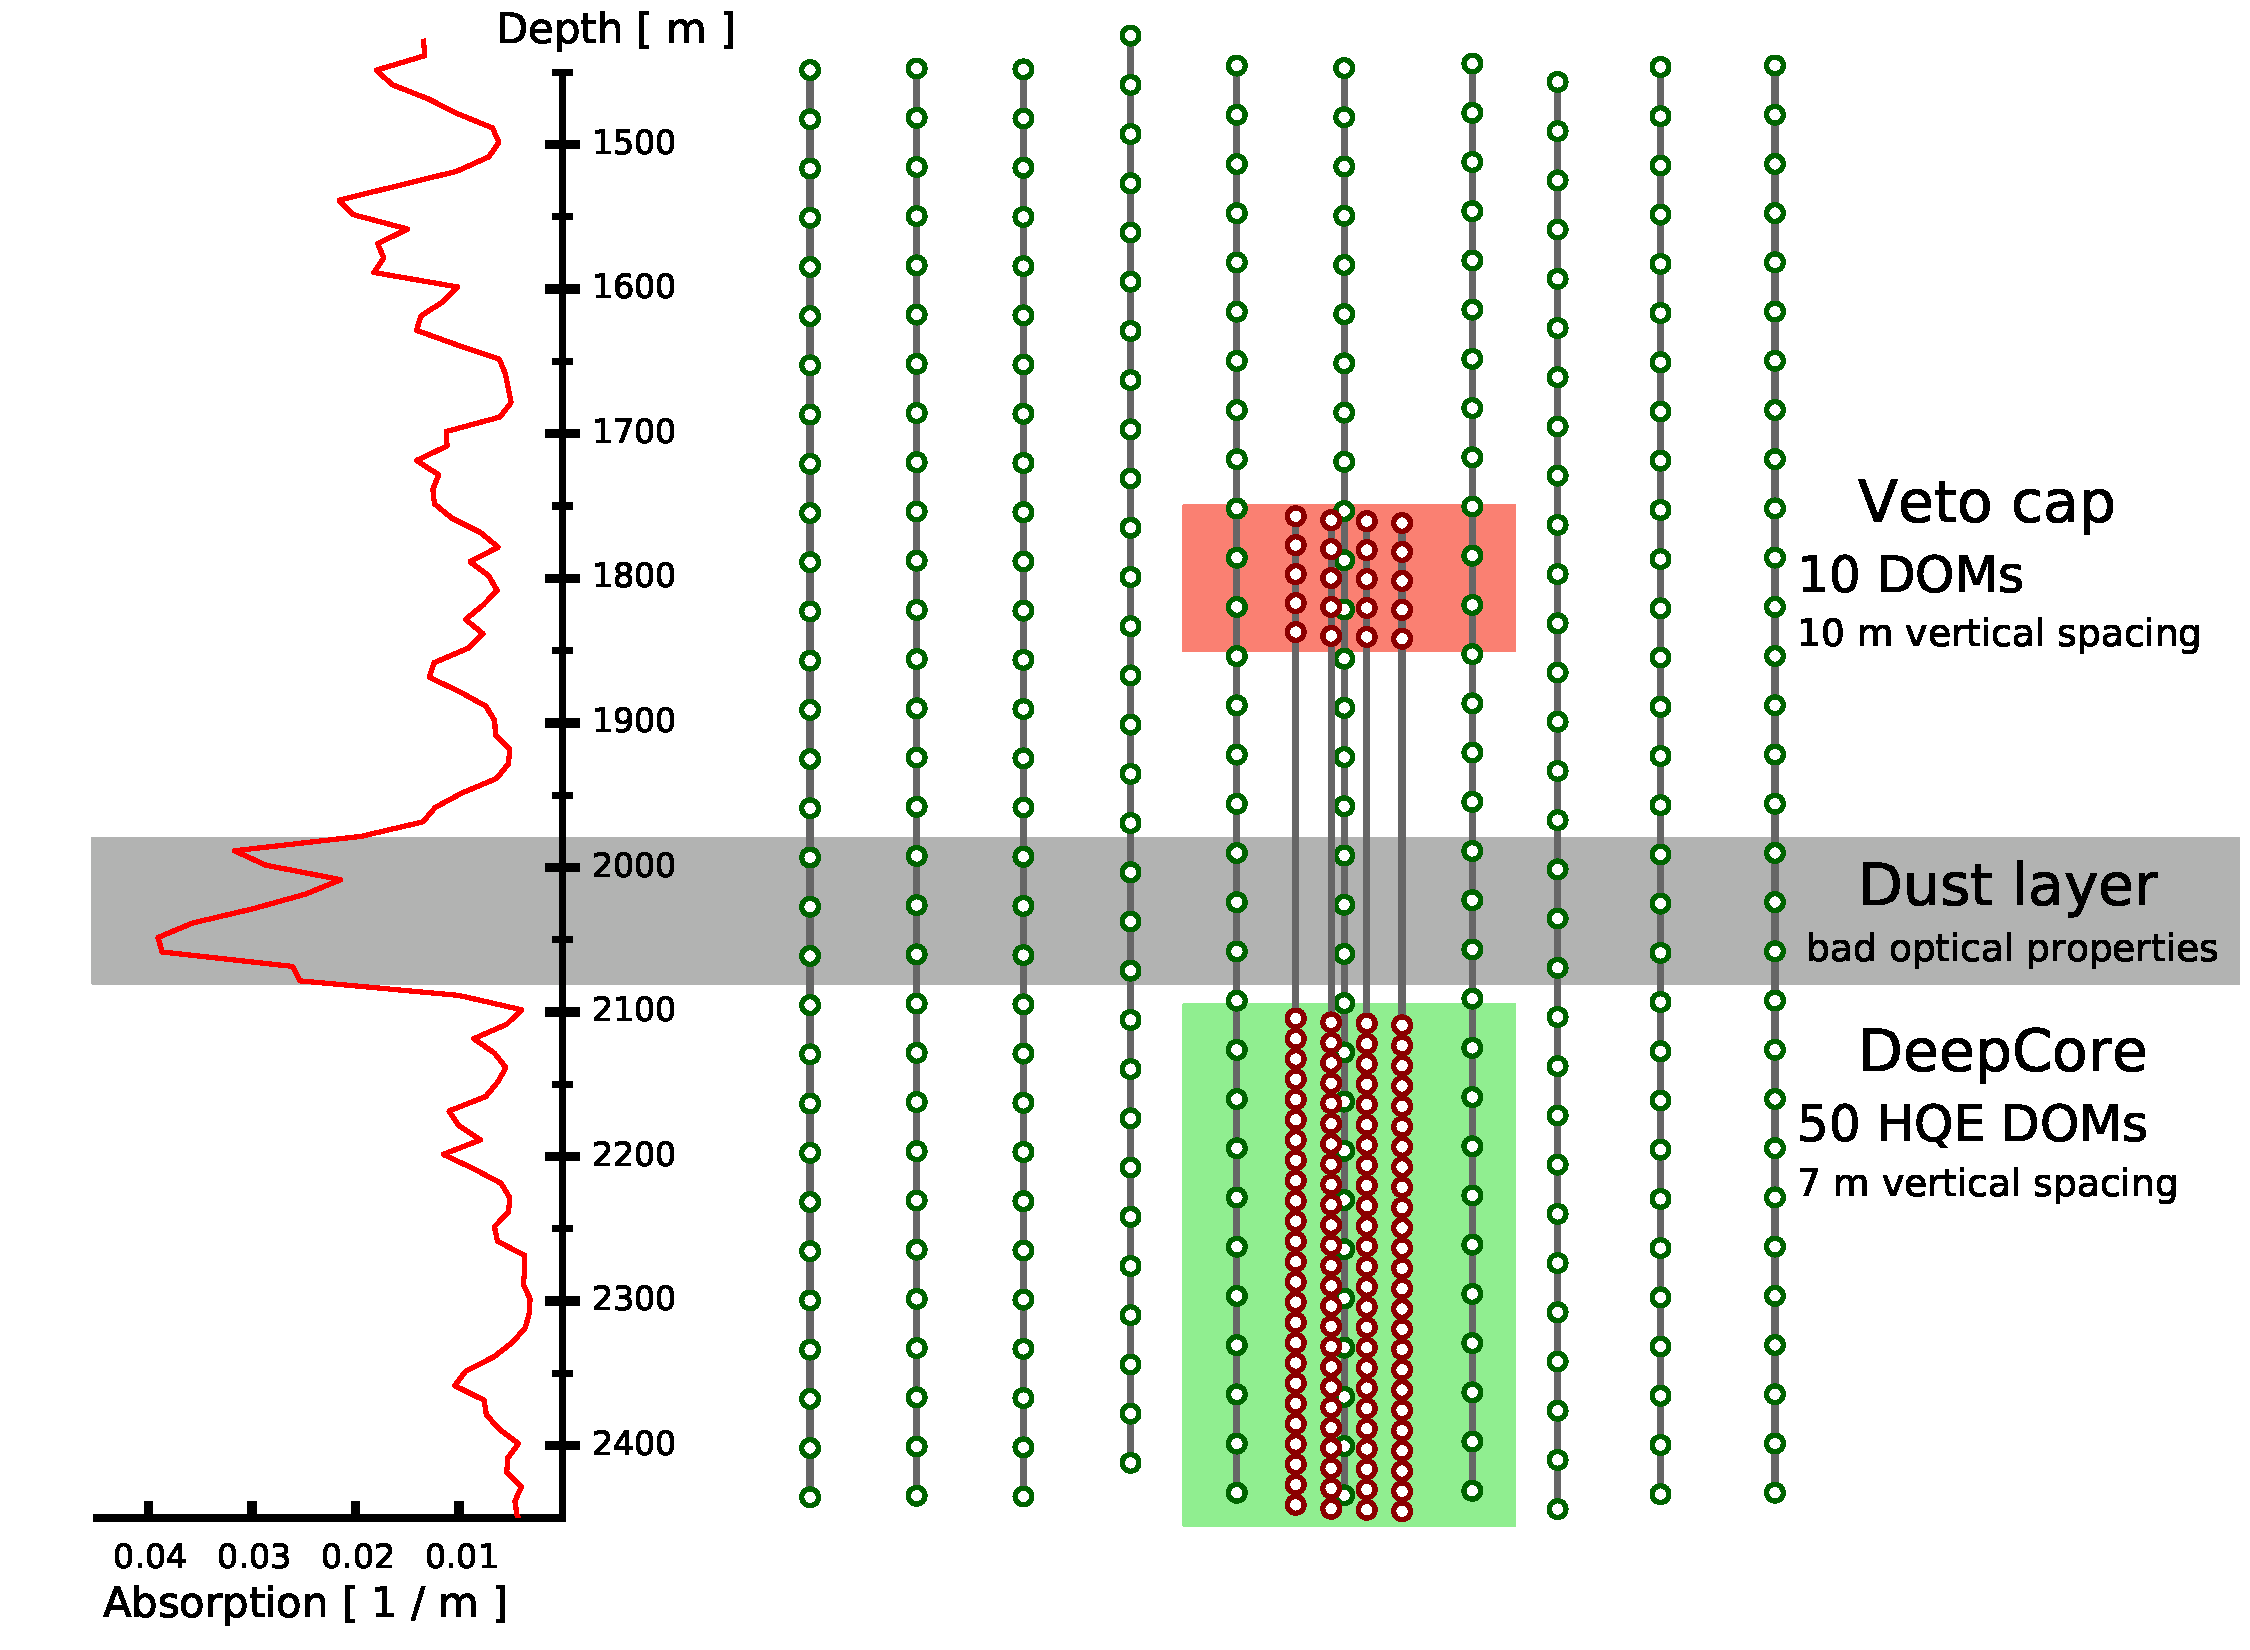
\includegraphics{figures/icecube_deepcore/DeepCore_sideview.pdf}
	\caption[IceCube side view]{Side view of IceCube and DeepCore showing the depth inverse of the absorption length (left panel) and the DOM positions around the dust layer.}
    \labfig{ic_dc_sidecut}
\end{figure}

The ice is instrumented by 5160 optical sensors called \textit{digital optical modules} (DOMs)~\sidecite{ABBASI2009294_data_acquisition}, which can detect the Cherenkov light produced by charged particles traveling through the ice. Each DOM is made of a spherical glass housing, containing a downward-facing \textit{photomultiplier tube (PMT)}, the main-board with control, readout, and processing-electronics, and a LED flasher-board for calibration purposes. The design and the individual components of a DOM can be seen in \reffig{DOM_design}.

The majority of PMTs are the \SI{10}{"} Hamamatsu R7081-02, which have a bialkali photocathode and are sensitive to wavelengths in the range of \SIrange{300}{650}{\nano\meter}, with a peak quantum efficiency of \SI{25}{\percent} at \SI{390}{\nano\meter}~\sidecite{2017JInst..12P3012A_Instrumentation_Systems}. The average dark count rate during operation in the ice is $\sim$\SI{300}{\hertz}. The DOM electronics measure the PMT voltage and control the gain. At a voltage crossing of the equivalent to \SI{0.25}{PE} the waveform readout is activated~\cite{ABBASI2009294_data_acquisition}. Only when either one of the nearest or next to nearest DOMs above or below also sees a voltage crossing within a \SI{1}{\micro\second} time window \sidenote{This is referred to as a \textit{hard local coincidence (HLC)}~\cite{ABBASI2009294_data_acquisition}.}, the voltages are digitized and sent to the ICL. Through the application of a waveform unfolding algorithm, called \textit{WaveDeform}~\sidecite{IceCube:2013dkx}, the waveforms are compressed, and the results are the reconstructed times and charges of the photo-electrons. This is the basis for all further IceCube data processing.

\begin{figure}
    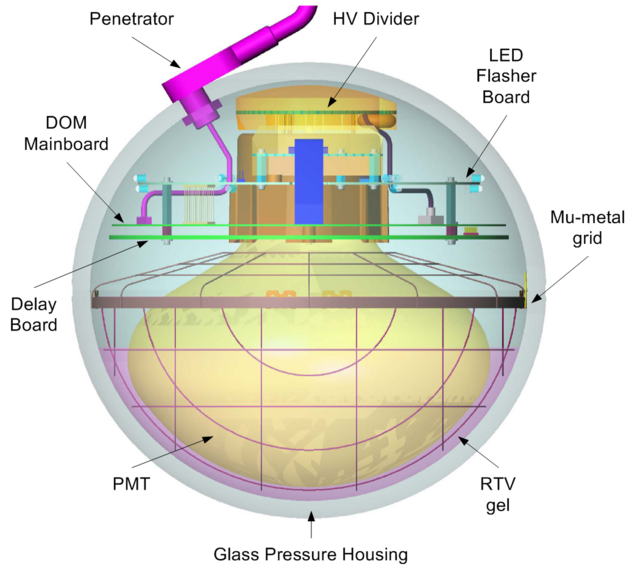
\includegraphics[width=0.6\textwidth]{figures/icecube_deepcore/DOM_schematic.png}
	\caption[Digital optical module (DOM)]{Design and components of a digital optical module (DOM)~\cite{ABBASI2009294_data_acquisition}}
    \labfig{DOM_design}
\end{figure}

The PMT is covered with a mu-metal grid (made from wire mesh), shielding the photocathode from Earth's magnetic field, and it is optically coupled to the glass sphere by RTV silicone gel. The glass sphere is a pressure vessel, designed to withstand both the constant ice pressure and the temporary pressure during the refreezing process of the water in the drill hole during deployment (peaking at around \SI{690}{\bar}). The sphere is held by a harness that connects the DOMs along a string and also guides the cable for power supply and communication beside them.

The flasher-board controls 12 LEDs that produce optical pulses with a wavelength of \SI{405}{\nano\meter}~\sidecite{2017JInst..12P3012A_Instrumentation_Systems}. The LEDs can be pulsed separately or in combination with variable output levels and pulse lengths. Using the known information of the light source positions and times this can be used for in-situ calibration of the detector by measuring absorption and scattering properties of the ice. Calibrating the absolute efficiency of the DOMs itself is more accurately done using minimum ionizing muons~\sidecite{JFeintzeig_phd, domeff_nick}, since the total amplitude of the LED light is not well known.


\subsection{IceCube Main-Array} \labsec{icecube}

\begin{figure}
    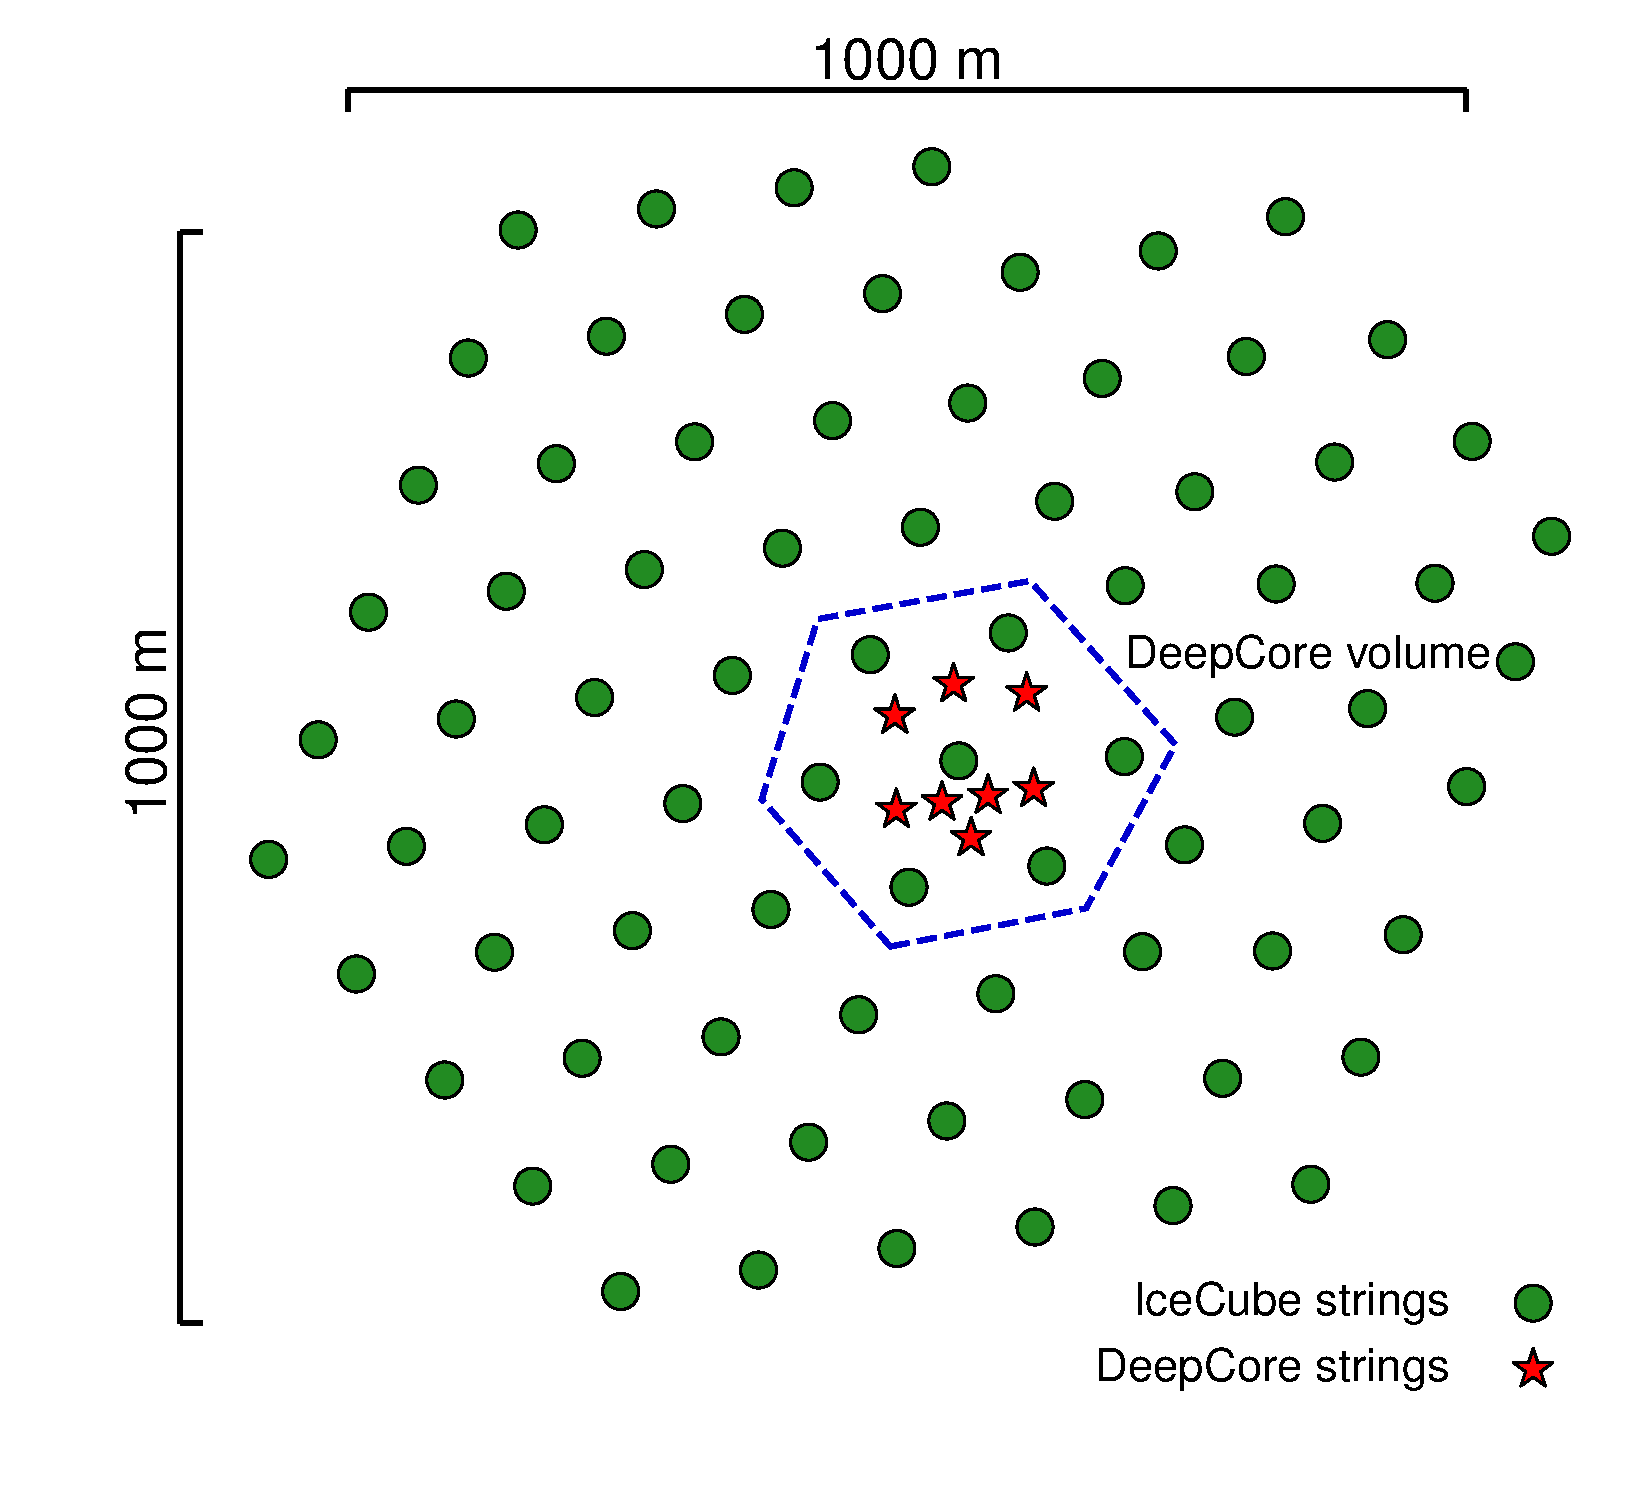
\includegraphics[trim={2.0cm, 1.5cm, 0, 0}, clip, width=0.65\linewidth]{figures/icecube_deepcore/icecube_top_view_bw.pdf}
    \caption[IceCube top view]{Top view of the IceCube array.}
    \labfig{icecube_top_view}
\end{figure}

The 78 strings that are arranged in a hexagonal pattern from the main part of the in-ice array, which is called \textit{IceCube}. With a $\sim$\SI{125}{\meter} horizontal spacing between the strings and a $\sim$\SI{17}{\meter} vertical spacing between DOMs, IceCube has a lower energy detection threshold of around \SI{100}{\gev}. IceCube was designed to detect high energy neutrinos of astrophysical origin.

The coordinate system that is used in IceCube is centered at 46500'E, 52200'N at an elevation of \SI{883.9}{\meter}~\cite{2017JInst..12P3012A_Instrumentation_Systems}. Per definition, it is a right-handed coordinate system where the y-axis points along the Prime Meridian (Grid North) towards Greenwich, UK, and the x-axis points \SI{90}{\degree} clockwise from the y-axis (Grid East). The z-axis is normal to the ice surface, pointing upwards. For IceCube analyses, depth is defined as the distance along the z axis from the ice surface, fixed at an elevation of \SI{2832}{\meter}.


\subsection{DeepCore Sub-Array} \labsec{deepcore}

The additional 8 strings form a denser sub-array of IceCube called \textit{DeepCore}~\sidecite{DeepCore_design_Abbasi2012615}. It is located at the bottom-center of the in-ice array and its \textit{fiducial volume} also includes the 7 surrounding IceCube strings as shown in \reffig{icecube_top_view}. The strings in this region have a closer average horizontal distance of about \SI{70}{\meter}. The lower 50 DeepCore DOMs on each string are placed in the region of clear ice below the dust layer between \SIrange{2100}{2450}{\meter} depth, where their vertical spacing is $\sim$\SI{7}{\meter}. The remaining 10 modules on each string are placed above the dust layer to be used as veto against atmospheric muons as can be seen in \reffig{ic_dc_sidecut}. Additionally, the DeepCore DOMs are equipped with higher quantum efficiency PMTs\sidenote{At \SI{400}{\nano\meter} they are \SI{35}{\percent} more efficient than the IceCube PMTs~\cite{DeepCore_design_Abbasi2012615}.}. The combination of the denser spacing, the high quantum efficiency modules, and the most favorable ice properties below the dust layer leads to a lower energy detection threshold of around \SI{5}{GeV}, allowing the more efficient observation of atmospheric neutrinos. This lower threshold enables measurements of neutrino oscillations and many other BSM studies such as dark matter searches, measurements of non-standard interactions, and searches for sterile neutrinos~\cite{DeepCore_design_Abbasi2012615}.


\section{Particle Propagation in Ice} \labsec{icecube_propagation}

Neutrinos interacting in the ice via DIS produce muons, electromagnetic showers, and hadronic showers, depending on their flavor and the interaction type. The particles produced in those processes mainly lose their energy through \textit{ionization}, \textit{bremsstrahlung}, \textit{pair production}, and the \textit{photo-nuclear interaction}. Electrically charged particles also emit Cherenkov light when traveling through the ice, which is the main observable in IceCube, but only contributes a small amount to the total energy loss.


\subsection{Cherenkov Effect} \labsec{cherenkov_effect}

The detection principle of IceCube DeepCore is based on the observation of Cherenkov photons that are emitted by the charged secondary particles produced in the neutrino interactions that were introduced in \refsec{neutrino_interactions}. The Cherenkov effect was first observed by Pavel Cherenkov in 1934~\sidecite{CherenkovPhysRev.52.378} and occurs when the charged particle travels faster than the phase velocity of light, therefore polarizing the medium. Upon de-excitation the molecules emit the received energy as photons in a spherical wavefront. Since the particle moves past this wavefront, the superposition of the spherical light emissions forms a cone, which is shown in blue in the bottom panel of \reffig{cherenkov_light_front}.

\begin{marginfigure}
    \centering
    \begin{tikzpicture}[scale=0.6]

        % slower than speed of light
        \draw[draw=none,fill=gray!60] (10,8) circle (0.1);
        \draw[draw=none,fill=gray!60] (10.5,8) circle (0.1);
        \draw[draw=none,fill=gray!60] (11,8) circle (0.1);
        \draw[draw=none,fill=gray!60] (11.5,8) circle (0.1);
        \draw[draw=none,fill=gray!60] (11.7,8) circle (0.1);
            
        \draw[tab_blue, line width=0.3mm] (10,8) circle (3.5);
        \draw[line width=0.3mm] (10.25,8) circle (3);
        \draw[line width=0.3mm] (10.5,8) circle (2.5);
        \draw[line width=0.3mm] (10.75,8) circle (2);
        \draw[line width=0.3mm] (11,8) circle (1.5);
        \draw[line width=0.3mm] (11.25,8) circle (1);
        \draw[line width=0.3mm] (11.5,8) circle (0.5);
        \draw[line width=0.3mm] (11.7,8) circle (0.1);

        \draw[tab_orange, line width=0.6mm] (10,8) -- (11.7,8);
        \draw[draw=none,fill=tab_orange] (11.8,8) -- +(210:0.45cm)arc (210:150:0.45cm) -- cycle;

        \draw[tab_orange, line width=0.6mm] (10,8) -- (11.9,11.00);

        \node[draw=tab_orange,line width=0.3mm] at (10.8,7.5) {$vt$};
        \node[draw=tab_orange,line width=0.3mm, rotate=59] at (10.5,9.7) {$ct$};

        \node[line width=0.3mm] at (10,4) {$v<c$};


        % faster than speed of light
        \draw[draw=none,fill=gray!60] (9,0) circle (0.1);
        \draw[draw=none,fill=gray!60] (10,0) circle (0.1);
        \draw[draw=none,fill=gray!60] (11,0) circle (0.1);
        \draw[draw=none,fill=gray!60] (12,0) circle (0.1);
        \draw[draw=none,fill=gray!60] (13,0) circle (0.1);
        \draw[draw=none,fill=gray!60] (13.5,0) circle (0.1);
        
        \draw[line width=0.3mm] (9,0) circle (2.5);
        \draw[line width=0.3mm] (10,0) circle (2);
        \draw[line width=0.3mm] (11,0) circle (1.5);
        \draw[line width=0.3mm] (12,0) circle (1);
        \draw[line width=0.3mm] (13,0) circle (0.5);
        \draw[line width=0.3mm] (13.5,0) circle (0.25);
        
        \draw[tab_blue, line width=0.3mm] (8,3.45) -- (14,0);
        \draw[tab_blue, line width=0.3mm] (8,-3.45) -- (14,0);
        
        \draw[tab_orange, line width=0.6mm] (9,0) -- (14,0);
        \draw[draw=none,fill=tab_orange] (14.1,0) -- +(210:0.45cm)arc (210:150:0.45cm) -- cycle;

        \draw[tab_orange, line width=0.6mm] (9,0) -- (10.3,2.15);
        
        \draw[tab_orange, line width=0.6mm] (9.8,0) arc (0:55:0.8cm);
        
        
        \node[] at (8.7,-0.6) {$\theta_c$};
        \draw[line width=0.2mm] (8.9,-0.4) -- (9.5,0.25);

        \node[draw=tab_orange,line width=0.3mm] at (10.5,-0.5) {$vt$};
        \node[draw=tab_orange,line width=0.3mm, rotate=59] at (9.0,1.0) {$ct$};

        \node[line width=0.3mm] at (10,-3.5) {$v>c$};

    \end{tikzpicture}
    \caption[Cherenkov light front]{Schematic depiction of the spherical light front produced by a particle traveling slower than the speed of light in the medium (top) and the formation of the Cherenkov light front produced by a charged particle traveling faster than the speed of light in the medium (bottom). The speed of light in the medium is $c$, $v$ is the speed of the particle, and $t$ is the time that has passed. Blue is the resulting wavefront, while the black circles are spherically emitted light at each position and the orange arrows show the direction of the particle.}
    \labfig{cherenkov_light_front}
\end{marginfigure}

Using trigonometry, the angle $\theta_c$ at which the Cherenkov light is emitted can be calculated as
\begin{equation}
    \theta_c = \arccos\Big(\frac{1}{\beta n}\Big)
    \;,
    \labeq{cherenkov_angle}
\end{equation}
where $\beta=v/c_\mathrm{vacuum}$ is the velocity of the particle in units of the speed of light, and $n$ is the refractive index of the medium that defines the speed of light in the medium $c=c_\mathrm{vacuum}*n$. When the particle velocity is close to the speed of light, the equation holds and the angle is only dependent on the refractive index of the medium. For ice, the refractive index is $n \approx 1.3$ and as a result $\theta_c \approx 41^\circ$~\cite{physics_of_ice_10.1093/acprof:oso/9780198518945.003.0009}.

The frequency of the emission depends on the charge $z$ and the wavelength-dependent index of refraction $n(\omega)$ and is given by the Frank-Tamm formula~\sidecite{frank, tamm}
\begin{equation}
    \frac{d^2N}{dxd\lambda} = \frac{2\pi\alpha z^2}{\lambda^2} \Big(1 - \frac{1}{\beta^2n(\omega)^2}\Big)
    \;,
    \labeq{frank_tamm}
\end{equation}
with $\alpha\approx1/137$ the fine structure constant, $\lambda$ the wavelength of the emitted light, and $x$ the path length traversed by the particle. Relativistic particles in ice produce roughly 250 photons per cm in the wavelength range of \SIrange[range-phrase={~-~}]{300}{500}{\nano\meter}~\cite{raedel_wiebusch_cherenkov_yield}.


\subsection{Energy Losses} \labsec{energy_loss}

Even though relativistic, charged particles traveling through matter produce Cherenkov radiation, their energy is mainly lost through other processes that are dependent on the particle type and energy. The exact principles of energy loss for the different types can broadly be categorized into the three groups: quasi-continuous energy loss by muons, electromagnetic cascades, and hadronic cascades.


\subsubsection{Muons}

Muons lose their energy by ionization, bremsstrahlung, pair production, and the photo-nuclear effect. The energy loss by ionization is the dominant process for muons above \SI{1}{\giga\electronvolt} and has a weak energy dependence given by~\cite{PDG_review_2022}
\begin{equation}
    \Bigl \langle -\frac{\mathrm{d}E}{\mathrm{d}x} \Bigr \rangle = a_I(E) + b_R(E) \cdot E
    \;,
    \labeq{radiative_losses}
\end{equation}
where $E$ is the energy, and $a_I(E)$ and $b_R(E) \cdot E$ are the energy loss by ionization and the combined radiative losses, respectively. In the energy range relevant for this work (below \SI{100}{\giga\electronvolt}), the parameters $a_I$ and $b_R$ only depend very weakly on energy and can be approximated by constants. The energy loss is then given by
\begin{equation}
    \Bigl \langle -\frac{\mathrm{d}E}{\mathrm{d}x} \Bigr \rangle = a + b \cdot E
    \;.
    \labeq{radiative_losses_simple}
\end{equation}
Based on this description, there is a critical energy which divides the regimes where ionization and radiative losses dominate. The critical energy is given by $E_\rm{crit} = a/b$ and for muons in ice it is $\sim$\SI{713}{\giga\electronvolt} (using $a \approx$ \SI{2.59}{\mega\electronvolt\cm^{-1}} and $b \approx$ \SI{3.63e-6}{\cm^{-1}}~\sidecite{2004hep.ph....7075C}). Since the energy range of interest is well below this critical energy, the range of a muon can easily be related to its energy by
\begin{equation}
    \langle L \rangle = \frac{E_0}{a}
    \;.
    \labeq{muon_range_approx}
\end{equation}
Measuring the length of a muon track therefore allows for an estimation of its energy if the full track is contained within the instrumented volume of IceCube. Using the given numbers, a \SI{30}{\giga\electronvolt} muon travels $\sim$\SI{116}{\meter}, which is well within the instrumented volume of IceCube, which spans across distances of up to \SI{1000}{\meter}. This approximate treatment does not take into account the stochastic nature of some energy losses. Bremsstrahlung and photo-nuclear interactions for example rarely occur, but when they do, they deposit a large portion of energy. A thorough investigation of the energy losses of muons in ice can be found in~\sidecite{LRaedel}.


\subsubsection{Electromagnetic Showers}

Photons as well as electrons and positrons are produced either directly in neutrino interactions or in secondary particle interactions. Above a critical energy $E_c$, they lose their energy through repeated pair production and bremsstrahlung emission forming an expanding, electromagnetic shower profile. The particles' energy reduces with every interaction and their number increases until they fall below the critical energy where ionization and excitation of surrounding atoms become the dominant energy loss processes for electrons and positrons. For photons the remaining energy is lost through the Compton effect and the photoelectric effect~\sidecite{PDG_review_2022}. Below the critical energy no new shower particles are produced.

Electromagnetic cascades can be characterized by the radiation length, $X_0$, after which electrons/positrons reduced their energy to $1/e$ of their initial energy. For photons, it is equivalent to $7/9$ of the mean free path of pair production. The critical energy for ice is $E_c \approx$ \SI{78}{\mega\electronvolt}, with a radiation length of $X_0 \approx$ \SI{39.3}{\centi\meter}~\sidecite{PhysRevD.98.030001}.

The radiation length governs the longitudinal shower profile and using $t=x/X_{0}$, the shower intensity can be described by a gamma distribution~\cite{PDG_review_2022}~\sidecite{em_gamma_distribution_Longo:1975wb}
\begin{equation}
    \frac{dE}{dt} = E_0b \frac{({bt})^{a-1} e^{-bt}}{\Gamma(a)}
    \;,
    \labeq{gamma_distribution}
\end{equation}
where $a$ and $b$ are parameters that have to be estimated from experiment, and $E_0$ is the initial shower energy. Based on the work from~\cite{LRaedel}, performed with \textsc{Geant4}~\sidecite{geant4}, the parameters for electromagnetic showers in ice are
\begin{subequations}
    \begin{align}
        e^-: \; a \approx 2.01 + 1.45 \log_{10} (E_0/\si{\giga\electronvolt}),\; & b \approx 0.63 \;, \\
        e^+: \; a \approx 2.00 + 1.46 \log_{10} (E_0/\si{\giga\electronvolt}),\; & b \approx 0.63 \;, \\
        \gamma: \; a \approx 2.84 + 1.34 \log_{10} (E_0/\si{\giga\electronvolt}),\; & b \approx 0.65 \;.
        \labeq{gamma_distribution_parameter}
    \end{align}
\end{subequations}
The maximum of the shower is at $t_{max} = (a-1)/b$ and the Cherenkov emission of the charged particles produced in the shower is peaked around the Cherenkov angle. \reffig{cherenkov_shower_profile} shows the angular shower profile of an EM shower from an electron, which peaks sharply around the Cherenkov angle.

\begin{marginfigure}
    \centering
    % This file was created with tikzplotlib v0.10.1.
\begin{tikzpicture}

\definecolor{darkgray176}{RGB}{176,176,176}
\definecolor{lightgray204}{RGB}{204,204,204}

\begin{axis}[
height=0.8\linewidth,
legend cell align={left},
legend style={
  fill opacity=0.8,
  draw opacity=1,
  text opacity=1,
  at={(0.03,0.97)},
  anchor=north west,
  draw=lightgray204
},
log basis y={10},
minor xtick={},
minor ytick={0.0002,0.0003,0.0004,0.0005,0.0006,0.0007,0.0008,0.0009,0.002,0.003,0.004,0.005,0.006,0.007,0.008,0.009,0.02,0.03,0.04,0.05,0.06,0.07,0.08,0.09,0.2,0.3,0.4,0.5,0.6,0.7,0.8,0.9,2,3,4,5,6,7,8,9,20,30,40,50,60,70,80,90,200,300,400,500,600,700,800,900},
tick align=outside,
tick pos=left,
width=\linewidth,
x grid style={darkgray176},
xlabel={\(\scriptstyle \cos(\vartheta)\)},
xmajorgrids,
xmin=-1.1, xmax=1.1,
xtick style={color=black},
xtick={-1.5,-1,-0.5,0,0.5,1,1.5},
xticklabels={
\(\scriptstyle -1.5\),
\(\scriptstyle -1\),
\(\scriptstyle -0.5\),
\(\scriptstyle 0\),
\(\scriptstyle 0.5\),
\(\scriptstyle 1\),
\(\scriptstyle 1.5\)
},
y grid style={darkgray176},
ylabel={\(\scriptstyle \frac{1}{N}\frac{\mathrm{d}n}{\mathrm{d}\Omega}\;(\mathrm{sr^{-1}})\)},
ymajorgrids,
ymin=0.00198893054244642, ymax=1.79304902414132,
ymode=log,
ytick style={color=black},
ytick={0.0001,0.001,0.01,0.1,1,10,100},
yticklabels={
  \(\scriptstyle {10^{-4}}\),
  \(\scriptstyle {10^{-3}}\),
  \(\scriptstyle {10^{-2}}\),
  \(\scriptstyle {10^{-1}}\),
  \(\scriptstyle {10^{0}}\),
  \(\scriptstyle {10^{1}}\),
  \(\scriptstyle {10^{2}}\)
}
]
% \addlegendimage{empty legend}
% \addlegendentry{\hspace{-.6cm}\(\scriptstyle Primary particle\)}
\addplot [very thick, tab_blue]
table {%
-1 0.00270979570996691
-0.989949748743719 0.00274568176844791
-0.979899497487437 0.00278221344276632
-0.969849246231156 0.0028194051401974
-0.959798994974874 0.00285727165740652
-0.949748743718593 0.00289582819293
-0.939698492462312 0.002935090360122
-0.92964824120603 0.00297507420058719
-0.919597989949749 0.00301579619812029
-0.909547738693467 0.00305727329317443
-0.899497487437186 0.00309952289788118
-0.889447236180904 0.00314256291164658
-0.879396984924623 0.00318641173734847
-0.869346733668342 0.00323108829816169
-0.85929648241206 0.00327661205503912
-0.849246231155779 0.00332300302487796
-0.839195979899497 0.00337028179940208
-0.829145728643216 0.00341846956479283
-0.819095477386935 0.00346758812210248
-0.809045226130653 0.00351765990848599
-0.798994974874372 0.00356870801928906
-0.78894472361809 0.00362075623103195
-0.778894472361809 0.00367382902533086
-0.768844221105528 0.00372795161380099
-0.758793969849246 0.00378314996398742
-0.748743718592965 0.00383945082637282
-0.738693467336683 0.00389688176251318
-0.728643216080402 0.00395547117435602
-0.718592964824121 0.00401524833479813
-0.708542713567839 0.00407624341954317
-0.698492462311558 0.00413848754032286
-0.688442211055276 0.00420201277954891
-0.678391959798995 0.00426685222646659
-0.668341708542714 0.00433304001488506
-0.658291457286432 0.00440061136256355
-0.648241206030151 0.00446960261233712
-0.638190954773869 0.00454005127507061
-0.628140703517588 0.00461199607453446
-0.618090452261307 0.00468547699430147
-0.608040201005025 0.00476053532676948
-0.597989949748744 0.0048372137244211
-0.587939698492462 0.00491555625343831
-0.577889447236181 0.00499560844979658
-0.5678391959799 0.00507741737797107
-0.557788944723618 0.00516103169239503
-0.547738693467337 0.00524650170181962
-0.537688442211055 0.00533387943673301
-0.527638190954774 0.0054232187200069
-0.517587939698492 0.00551457524094897
-0.507537688442211 0.0056080066329506
-0.49748743718593 0.00570357255493209
-0.487437185929648 0.00580133477679948
-0.477386934673367 0.00590135726914189
-0.467336683417085 0.00600370629741217
-0.457286432160804 0.0061084505208506
-0.447236180904523 0.00621566109642723
-0.437185929648241 0.00632541178809819
-0.42713567839196 0.00643777908168967
-0.417085427135678 0.00655284230574558
-0.407035175879397 0.00667068375869704
-0.396984924623116 0.00679138884273666
-0.386934673366834 0.00691504620480722
-0.376884422110553 0.00704174788514251
-0.366834170854271 0.00717158947382927
-0.35678391959799 0.00730467027589214
-0.346733668341708 0.0074410934854396
-0.336683417085427 0.00758096636944745
-0.326633165829146 0.0077244004617986
-0.316582914572864 0.00787151176824312
-0.306532663316583 0.0080224209829917
-0.296482412060301 0.00817725371770887
-0.28643216080402 0.00833614074373032
-0.276381909547739 0.00849921824839105
-0.266331658291457 0.00866662810641917
-0.256281407035176 0.0088385181674243
-0.246231155778894 0.00901504256058975
-0.236180904522613 0.00919636201776539
-0.226130653266332 0.00938264421625311
-0.21608040201005 0.0095740641426814
-0.206030150753769 0.00977080447947795
-0.195979899497487 0.00997305601557417
-0.185929648241206 0.0101810180831098
-0.175879396984925 0.0103948990220547
-0.165829145728643 0.0106149166748261
-0.155778894472362 0.0108412989131575
-0.14572864321608 0.0110742841996714
-0.135678391959799 0.0113141221868181
-0.125628140703518 0.0115610743560839
-0.115577889447236 0.0118154147006228
-0.105527638190955 0.0120774304547576
-0.0954773869346733 0.0123474228741045
-0.085427135678392 0.0126257080704248
-0.0753768844221105 0.0129126179056865
-0.0653266331658291 0.0132085009502441
-0.0552763819095478 0.0135137235105104
-0.0452261306532663 0.0138286707320131
-0.035175879396985 0.0141537477843051
-0.0251256281407035 0.0144893811348354
-0.0150753768844221 0.0148360199195975
-0.00502512562814073 0.0151941374191663
0.00502512562814061 0.0155642326496143
0.0150753768844221 0.0159468320787846
0.0251256281407035 0.0163424914795012
0.035175879396985 0.0167517979325291
0.0452261306532664 0.0171753719934818
0.0552763819095476 0.0176138700394269
0.0653266331658291 0.0180679868126891
0.0753768844221105 0.0185384581813153
0.085427135678392 0.0190260641378932
0.0954773869346734 0.0195316320609182
0.105527638190955 0.0200560402657496
0.115577889447236 0.0206002218754172
0.125628140703518 0.0211651690451993
0.135678391959799 0.0217519375790622
0.14572864321608 0.022361651980798
0.155778894472362 0.0229955109881295
0.165829145728643 0.0236547936442626
0.175879396984925 0.0243408659685004
0.185929648241206 0.0250551882957267
0.195979899497488 0.0257993233640178
0.206030150753769 0.0265749452405507
0.21608040201005 0.0273838491886102
0.226130653266332 0.0282279625931581
0.236180904522613 0.0291093570794933
0.246231155778895 0.0300302619794334
0.256281407035176 0.030993079322741
0.266331658291457 0.03200040055884
0.276381909547739 0.0330550252460245
0.28643216080402 0.0341599819833132
0.296482412060302 0.0353185519050526
0.306532663316583 0.0365342951117703
0.316582914572864 0.0378110804744502
0.326633165829146 0.0391531193255863
0.336683417085427 0.040565003641884
0.346733668341709 0.0420517494338256
0.35678391959799 0.0436188461909371
0.366834170854271 0.0452723133940923
0.376884422110553 0.0470187653046993
0.386934673366834 0.0488654854842812
0.396984924623116 0.0508205127985405
0.407035175879397 0.0528927410327426
0.417085427135678 0.055092034710039
0.42713567839196 0.057429364287307
0.437185929648241 0.0599169646387465
0.447236180904523 0.0625685216719253
0.457286432160804 0.0653993931161115
0.467336683417085 0.0684268710625494
0.477386934673367 0.0716704958356979
0.487437185929648 0.0751524333921324
0.49748743718593 0.0788979319015025
0.507537688442211 0.0829358777746636
0.517587939698493 0.0872994776151978
0.527638190954774 0.0920271010294813
0.537688442211055 0.0971633308874874
0.547738693467337 0.102760283897193
0.557788944723618 0.108879287382879
0.5678391959799 0.115593031243989
0.577889447236181 0.122988362403445
0.587939698492462 0.131169960953129
0.597989949748744 0.140265246331153
0.608040201005025 0.15043103123486
0.618090452261307 0.16186271048248
0.628140703517588 0.17480721310861
0.638190954773869 0.189581691206729
0.648241206030151 0.20660122497593
0.658291457286432 0.226421210798552
0.668341708542714 0.249804685334967
0.678391959798995 0.277834184784676
0.688442211055276 0.312108201800071
0.698492462311558 0.355111292696392
0.708542713567839 0.410978453421262
0.718592964824121 0.487286890541685
0.728643216080402 0.60012697327905
0.738693467336683 0.793910321136359
0.748743718592965 1.3160586073339
0.758793969849246 1.02808069276863
0.768844221105528 0.705773104929006
0.778894472361809 0.551690720919282
0.78894472361809 0.455470028921774
0.798994974874372 0.388094231142621
0.809045226130653 0.337707570767511
0.819095477386935 0.298358445355108
0.829145728643216 0.266664676520879
0.839195979899497 0.240535857090921
0.849246231155779 0.218598677952748
0.85929648241206 0.199907969806359
0.869346733668342 0.183788893273284
0.879396984924623 0.169745057977341
0.889447236180904 0.157402218673429
0.899497487437186 0.146472295437764
0.909547738693467 0.13672956196271
0.919597989949749 0.127994411299455
0.92964824120603 0.120122001115478
0.939698492462312 0.112994133285036
0.949748743718593 0.106513332049104
0.959798994974874 0.100598450200823
0.969849246231156 0.0951813583735468
0.979899497487437 0.090204415681687
0.989949748743719 0.0856185130166524
1 0.0813815420878193
};
\addlegendentry{\(\scriptstyle e^-\)}
\addplot [very thick, tab_orange]
table {%
-1 0.00789216051649666
-0.989949748743719 0.00794087635636688
-0.979899497487437 0.00799046060080033
-0.969849246231156 0.00804093213801919
-0.959798994974874 0.00809231034956343
-0.949748743718593 0.00814461512551476
-0.939698492462312 0.00819786688026744
-0.92964824120603 0.00825208656886829
-0.919597989949749 0.00830729570394975
-0.909547738693467 0.00836351637328043
-0.899497487437186 0.0084207712579593
-0.889447236180904 0.00847908365128039
-0.879396984924623 0.00853847747829651
-0.869346733668342 0.00859897731611185
-0.85929648241206 0.00866060841493438
-0.849246231155779 0.00872339671992113
-0.839195979899497 0.00878736889385044
-0.829145728643216 0.00885255234065718
-0.819095477386935 0.00891897522986894
-0.809045226130653 0.00898666652198258
-0.798994974874372 0.0090556559948231
-0.78894472361809 0.00912597427092828
-0.778894472361809 0.00919765284600533
-0.768844221105528 0.00927072411850768
-0.758793969849246 0.00934522142038275
-0.748743718592965 0.00942117904904423
-0.738693467336683 0.00949863230062473
-0.728643216080402 0.00957761750456841
-0.718592964824121 0.00965817205962519
-0.708542713567839 0.00974033447131266
-0.698492462311558 0.00982414439091419
-0.688442211055276 0.00990964265608621
-0.678391959798995 0.00999687133315109
-0.668341708542714 0.0100858737611565
-0.658291457286432 0.0101766945977864
-0.648241206030151 0.0102693798672131
-0.638190954773869 0.0103639770099861
-0.628140703517588 0.0104605349350563
-0.618090452261307 0.0105591040740432
-0.608040201005025 0.0106597364378548
-0.597989949748744 0.0107624856757796
-0.587939698492462 0.0108674071371743
-0.577889447236181 0.0109745579358802
-0.5678391959799 0.0110839970175068
-0.557788944723618 0.0111957852297315
-0.547738693467337 0.0113099853957697
-0.537688442211055 0.0114266623911839
-0.527638190954774 0.0115458832242044
-0.517587939698492 0.0116677171197494
-0.507537688442211 0.0117922356073411
-0.49748743718593 0.0119195126131274
-0.487437185929648 0.0120496245562312
-0.477386934673367 0.0121826504496634
-0.467336683417085 0.0123186720060495
-0.457286432160804 0.0124577737484374
-0.447236180904523 0.0126000431264682
-0.437185929648241 0.0127455706382125
-0.42713567839196 0.0128944499579918
-0.417085427135678 0.0130467780705269
-0.407035175879397 0.0132026554117768
-0.396984924623116 0.013362186016856
-0.386934673366834 0.0135254776754425
-0.376884422110553 0.0136926420951192
-0.366834170854271 0.0138637950731175
-0.35678391959799 0.0140390566769668
-0.346733668341708 0.0142185514345872
-0.336683417085427 0.0144024085343986
-0.326633165829146 0.0145907620360627
-0.316582914572864 0.0147837510925123
-0.306532663316583 0.0149815201839753
-0.296482412060301 0.0151842193647459
-0.28643216080402 0.0153920045235134
-0.276381909547739 0.0156050376581157
-0.266331658291457 0.0158234871656503
-0.256281407035176 0.0160475281489437
-0.246231155778894 0.0162773427404552
-0.236180904522613 0.0165131204447723
-0.226130653266332 0.0167550585009444
-0.21608040201005 0.0170033622659962
-0.206030150753769 0.0172582456210662
-0.195979899497487 0.0175199314017323
-0.185929648241206 0.0177886518542055
-0.175879396984925 0.0180646491192131
-0.165829145728643 0.0183481757455348
-0.155778894472362 0.0186394952353194
-0.14572864321608 0.0189388826234856
-0.135678391959799 0.0192466250936987
-0.125628140703518 0.0195630226336309
-0.115577889447236 0.0198883887324402
-0.105527638190955 0.0202230511236558
-0.0954773869346733 0.0205673525769393
-0.085427135678392 0.0209216517424914
-0.0753768844221105 0.0212863240522157
-0.0653266331658291 0.0216617626821167
-0.0552763819095478 0.0220483795808203
-0.0452261306532663 0.022446606569557
-0.035175879396985 0.0228568965194424
-0.0251256281407035 0.0232797246124452
-0.0150753768844221 0.0237155896930427
-0.00502512562814073 0.0241650157182394
0.00502512562814061 0.0246285533143807
0.0150753768844221 0.0251067814500269
0.0251256281407035 0.025600309235087
0.035175879396985 0.0261097778574502
0.0452261306532664 0.0266358626695118
0.0552763819095476 0.0271792754382893
0.0653266331658291 0.0277407667742745
0.0753768844221105 0.0283211287557975
0.085427135678392 0.0289211977675074
0.0954773869346734 0.0295418575736295
0.105527638190955 0.0301840426489816
0.115577889447236 0.0308487417933436
0.125628140703518 0.0315370020577348
0.135678391959799 0.032249933014505
0.14572864321608 0.032988711406942
0.155778894472362 0.0337545862184264
0.165829145728643 0.0345488842060796
0.175879396984925 0.0353730159494754
0.185929648241206 0.0362284824714063
0.195979899497488 0.0371168824950634
0.206030150753769 0.0380399204104475
0.21608040201005 0.0389994150325696
0.226130653266332 0.0399973092452438
0.236180904522613 0.0410356806372771
0.246231155778895 0.0421167532529549
0.256281407035176 0.0432429105962605
0.266331658291457 0.0444167100487352
0.276381909547739 0.0456408988848156
0.28643216080402 0.0469184320965592
0.296482412060302 0.048252492272703
0.306532663316583 0.0496465118159931
0.316582914572864 0.0511041978289106
0.326633165829146 0.0526295600528103
0.336683417085427 0.0542269423109717
0.346733668341709 0.0559010579844757
0.35678391959799 0.0576570301440859
0.366834170854271 0.0595004370751213
0.376884422110553 0.0614373640703005
0.386934673366834 0.0634744625336283
0.396984924623116 0.0656190176441357
0.407035175879397 0.0678790260813921
0.417085427135678 0.0702632856277359
0.42713567839196 0.0727814988515182
0.437185929648241 0.075444393562777
0.447236180904523 0.0782638633461016
0.457286432160804 0.0812531322528268
0.467336683417085 0.0844269487270227
0.477386934673367 0.0878018151159875
0.487437185929648 0.0913962607705643
0.49748743718593 0.0952311689042153
0.507537688442211 0.099330170235027
0.517587939698493 0.103720120240028
0.527638190954774 0.108431681976416
0.537688442211055 0.113500043406718
0.547738693467337 0.118965807795903
0.557788944723618 0.124876109212345
0.5678391959799 0.131286024264284
0.577889447236181 0.138260378736104
0.587939698492462 0.145876088183355
0.597989949748744 0.154225231976222
0.608040201005025 0.163419152664381
0.618090452261307 0.173594017226095
0.628140703517588 0.18491850963698
0.638190954773869 0.197604710766709
0.648241206030151 0.211923886477276
0.658291457286432 0.228230096197278
0.668341708542714 0.246996774450726
0.678391959798995 0.26887589872466
0.688442211055276 0.294798880744473
0.698492462311558 0.32616049150544
0.708542713567839 0.36518484083375
0.718592964824121 0.41574694864329
0.728643216080402 0.48557899814055
0.738693467336683 0.594309602959545
0.748743718592965 0.835983791833013
0.758793969849246 0.710693050136147
0.768844221105528 0.546432769731992
0.778894472361809 0.456265851073738
0.78894472361809 0.395022749599503
0.798994974874372 0.349420179510256
0.809045226130653 0.313615587438124
0.819095477386935 0.284503587518325
0.829145728643216 0.260234102069794
0.839195979899497 0.239616407766554
0.849246231155779 0.221839941214909
0.85929648241206 0.206328850988604
0.869346733668342 0.192660020219313
0.879396984924623 0.180513958673293
0.889447236180904 0.169643916401901
0.899497487437186 0.159855667085849
0.909547738693467 0.150993826949325
0.919597989949749 0.142932331066801
0.92964824120603 0.135567640702552
0.939698492462312 0.128813795145942
0.949748743718593 0.122598739772099
0.959798994974874 0.116861556117663
0.969849246231156 0.111550341625584
0.979899497487437 0.10662056525917
0.989949748743719 0.102033776999246
1 0.0977565841356766
};
\addlegendentry{\(\scriptstyle \pi^+\)}
\addplot [black, dashed, forget plot]
table {%
0.75187969924812 0.00198893054244642
0.75187969924812 1.79304902414132
};
\end{axis}

\end{tikzpicture}

    \caption[Angular profile of EM and hadronic shower]{Angular Cherenkov emission profile of an EM shower ($e^-$) and a hadronic cascade ($\pi^+$), taken from~\cite{ATrettin_phd}, based on the parameterizations from~\cite{LRaedel}.}
    \labfig{cherenkov_shower_profile}
\end{marginfigure}


\subsubsection{Hadronic Showers} \labsec{hadronic_showers}

In DIS interactions, a cascade is always produced by the hadrons coming from the target nucleus that is breaking apart. The cascade is a result of secondary particles produced in strong interactions between the hadrons and the traversed matter. The charged particles produced in the shower will emit Cherenkov radiation, while neutral particles will be invisible to the detector. There is also an electromagnetic component of the shower, for example, due to the decay of neutral pions into photons. Hadronic showers of the same energy as electromagnetic showers have larger fluctuations in energy deposition and shape, since they depend on the produced particle types. Hadrons also have a higher energy threshold for Cherenkov light production, because of their higher mass. Based on~\cite{LRaedel}~\sidecite{GABRIEL1994336}, the visible electromagnetic fraction of hadronic showers can be parameterized as
\begin{equation}
    F(E_0) = \frac{T_\mathrm{hadron}}{T_\mathrm{EM}} = 1 - (1 - f_0)\Big(\frac{E_0}{E_s}\Big)^{-m}
    \;,
    \labeq{hadronic_shower_fraction}
\end{equation}
where $T_\mathrm{hadron/EM}$ is the total track length of a hadronic/electromagnetic shower with the same energy, $f_0$ is the ratio of hadronic and electromagnetic light yield, $E_0$ is the initial energy, and $E_s$ is an energy scale. The parameter $m$ is a free model parameter. The ratio $F(E_0)$ increases with energy, but is always smaller than $1$. The variance of this distribution is given by
\begin{equation}
    \sigma_F(E_0) = \sigma_0 \log(E_0)^{-\gamma}
    \;.
    \labeq{hadronic_shower_fraction_variance}
\end{equation}
The parameters $m$, $E_s$, and $f_0$ were estimated by fitting the model to the results of Geant4 simulations. Cherenkov light from hadronic showers also peaks around the Cherenkov angle, but the angular distribution is more smeared out, due to the variations in particle type and their energy depositions. This can be seen in \reffig{cherenkov_shower_profile}, where the angular emission profile of a shower from a $\pi^+$ is shown as an example for a hadronic shower.


\section{Event Morphologies} \labsec{icecube_signatures}

The event morphologies produced by particles detected in IceCube are combinations of the three energy loss types described in \refsec{energy_loss}, e.g. \textit{cascades} from electromagnetic and hadronic showers and elongated \textit{tracks} from muons traveling through the detector. \reftab{interactions_vs_signatures} gives an overview of the possible event signatures from standard model interactions. The unique double-cascade signature of the HNL, introduced in \refsec{double_cascade_morphology} is not listed again in the table.

\begin{table}[h]
    \small
    \begin{center}
        \begin{tabular}{ m{1.8cm} m{2.0cm} m{3.0cm} m{1.8cm} }
        % \begin{tabular}{ l l l l }

            \hline\hline

            \textbf{Interaction} & \multicolumn{2}{c}{\textbf{Secondary particles}} &\textbf{Signature} \\

            \hline\hline

            \multirow{2}{*}[-1.5em]{CC $\overset{(-)}{\nu_\mu}$ }
            & 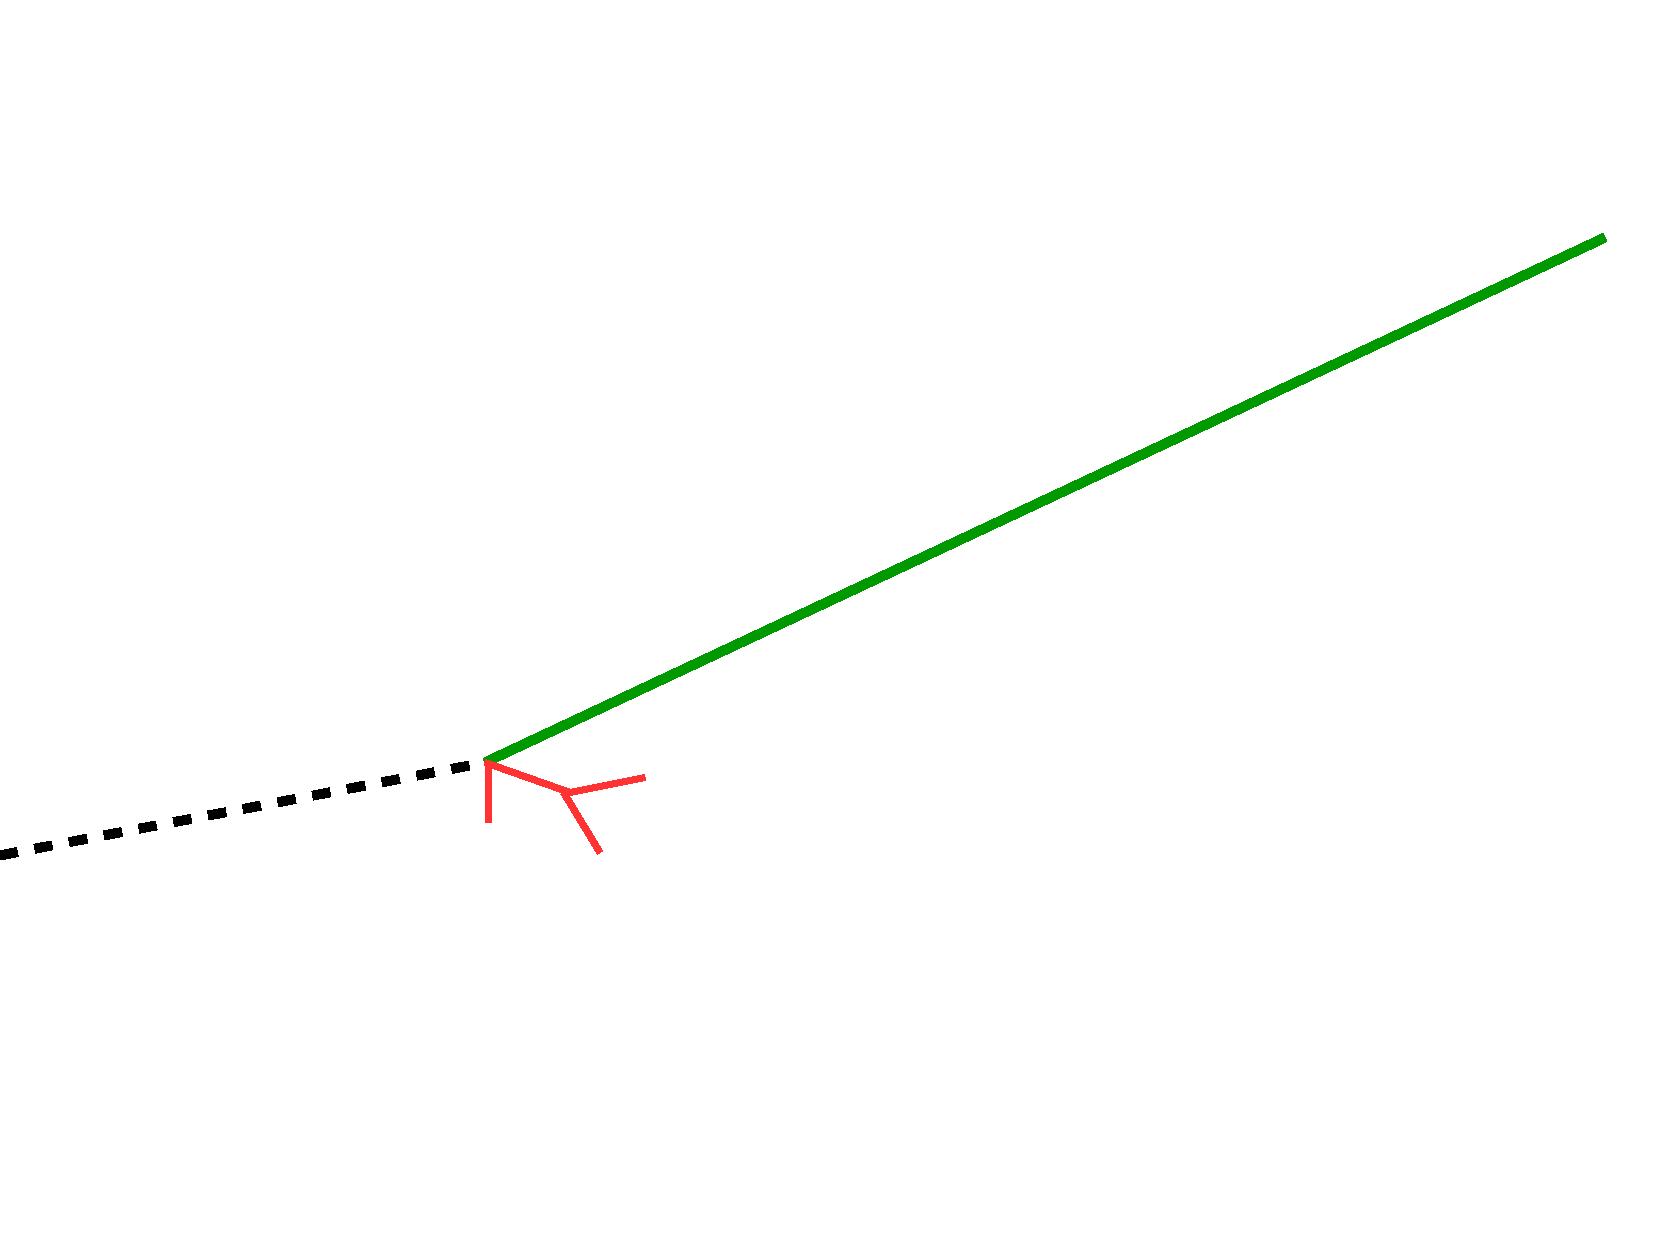
\includegraphics[width=2cm]{figures/neutrinos_properties/interaction_schematics/numu_CC_muon_only.pdf} 
            & $\mu^\pm$ track 
            & Track-only \\

            \cmidrule{2-4} 
            &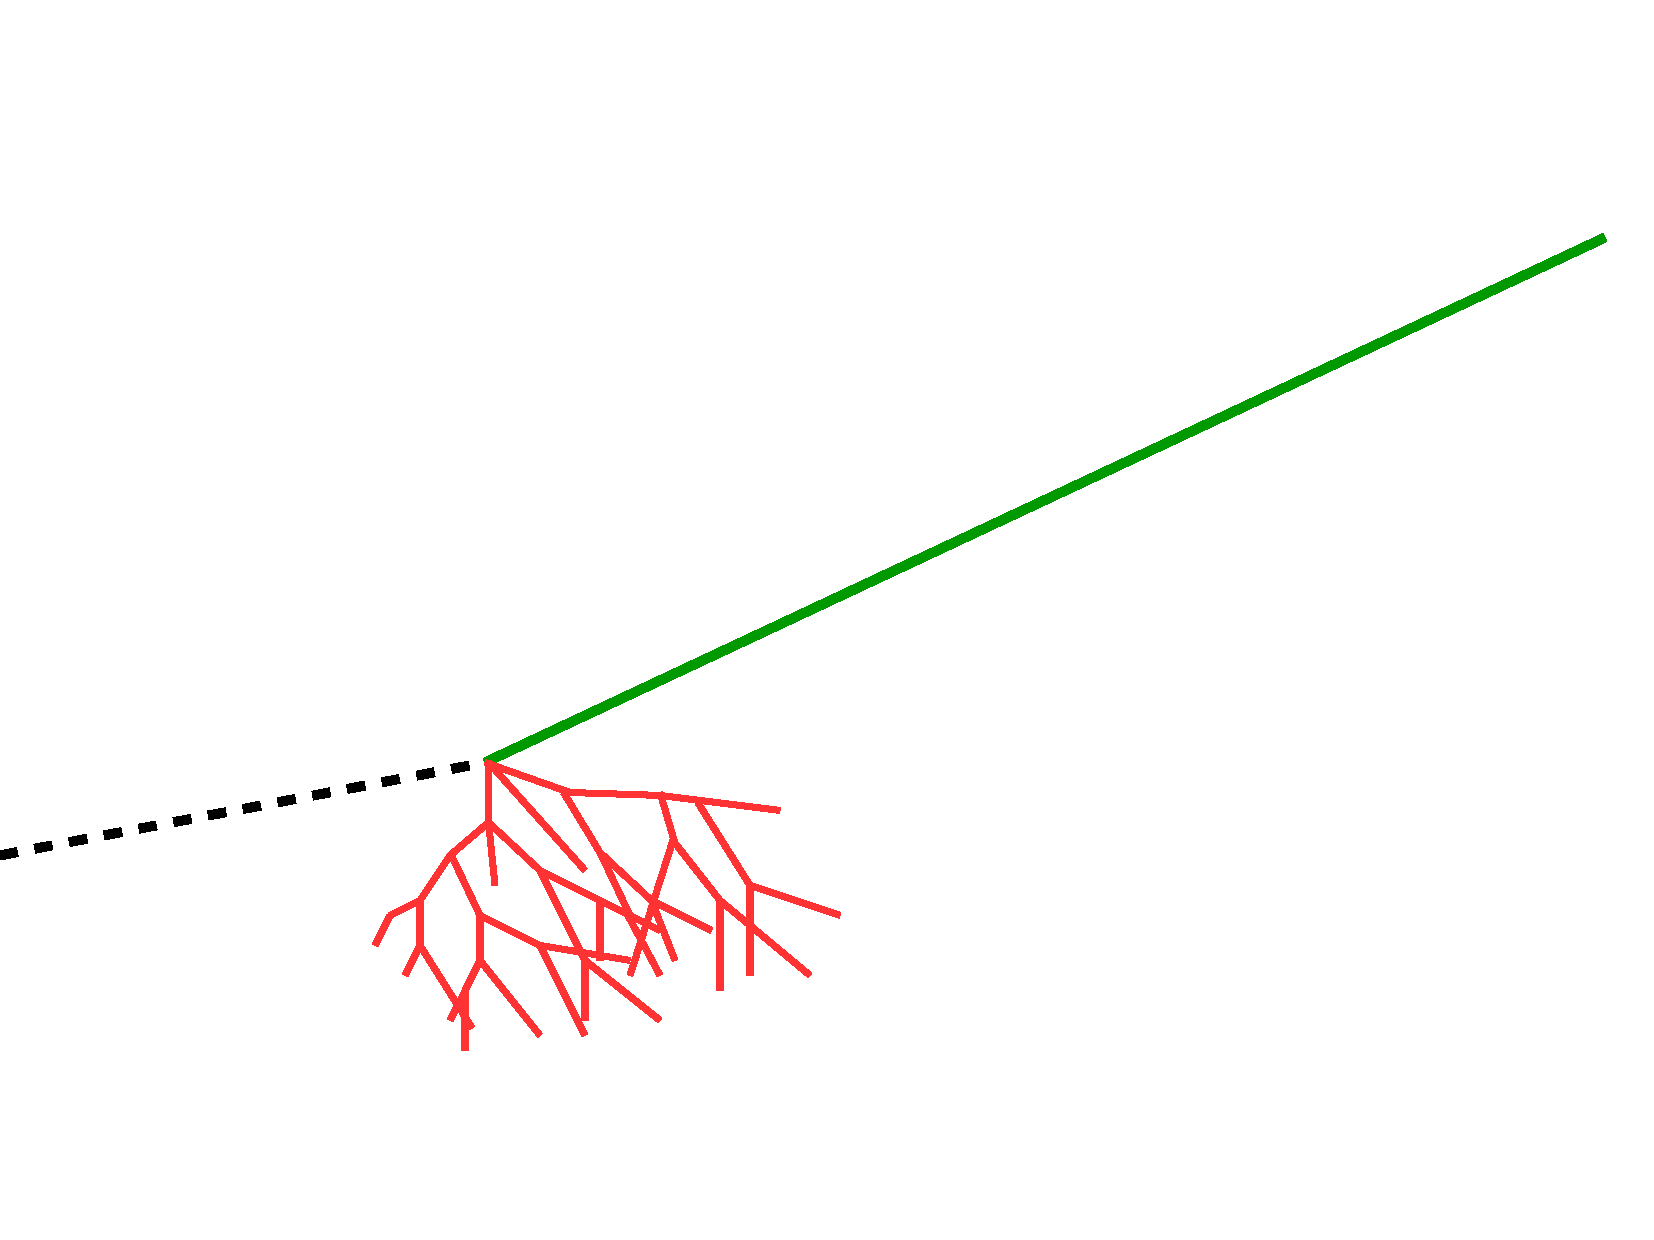
\includegraphics[width=2cm]{figures/neutrinos_properties/interaction_schematics/numu_CC_track_cascade.pdf}  
            & $\mu^\pm$ track and hadrons 
            & \multirow{2}{*}[-1.3em] {Cascade + track} \\

            \cmidrule{1-3}

            \multirow{2}{*}[-1.5em]{CC $\overset{(-)}{\nu_\tau}$ }
            &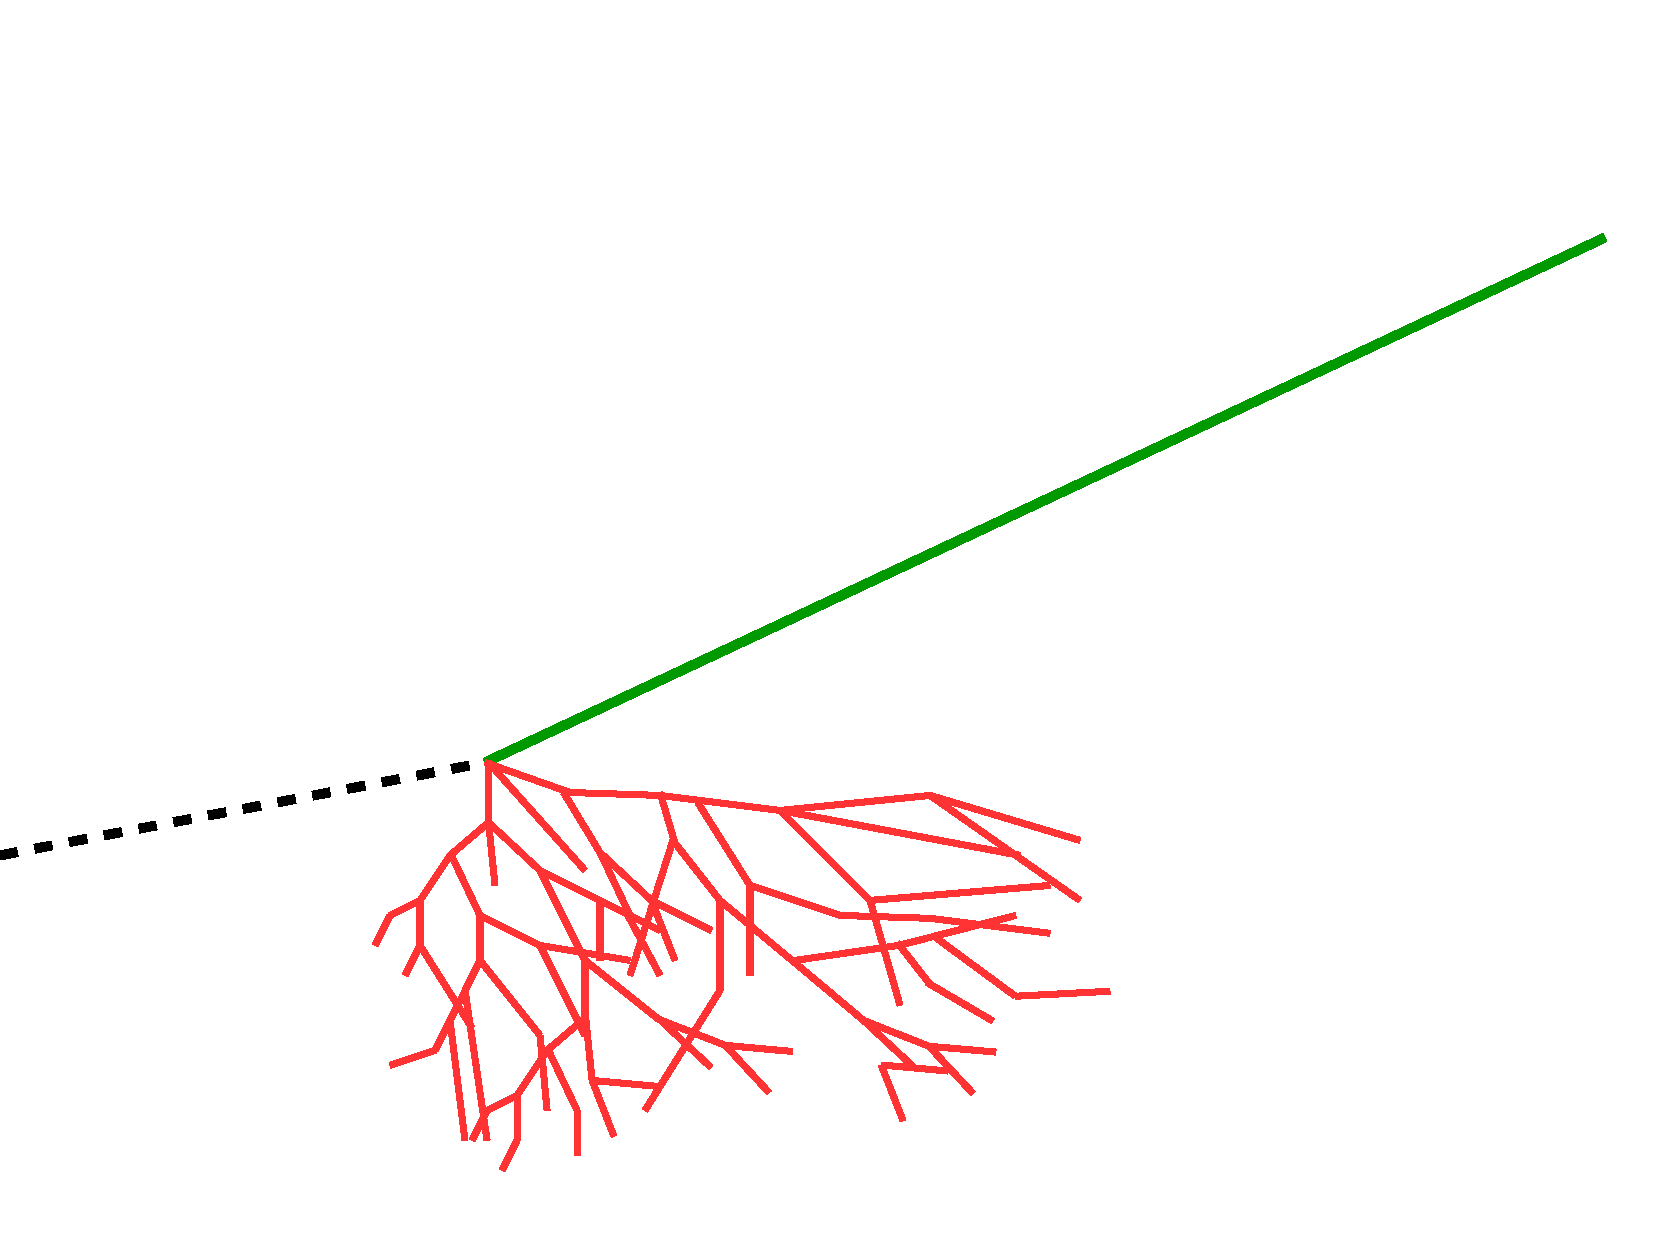
\includegraphics[width=2cm]{figures/neutrinos_properties/interaction_schematics/nutau_CC_track_cascade.pdf} 
            & $\tau^\pm$ decaying into $\mu^\pm$ ($\sim$17\% BR), hadrons 
            & \\

            \cmidrule{2-4}

            & 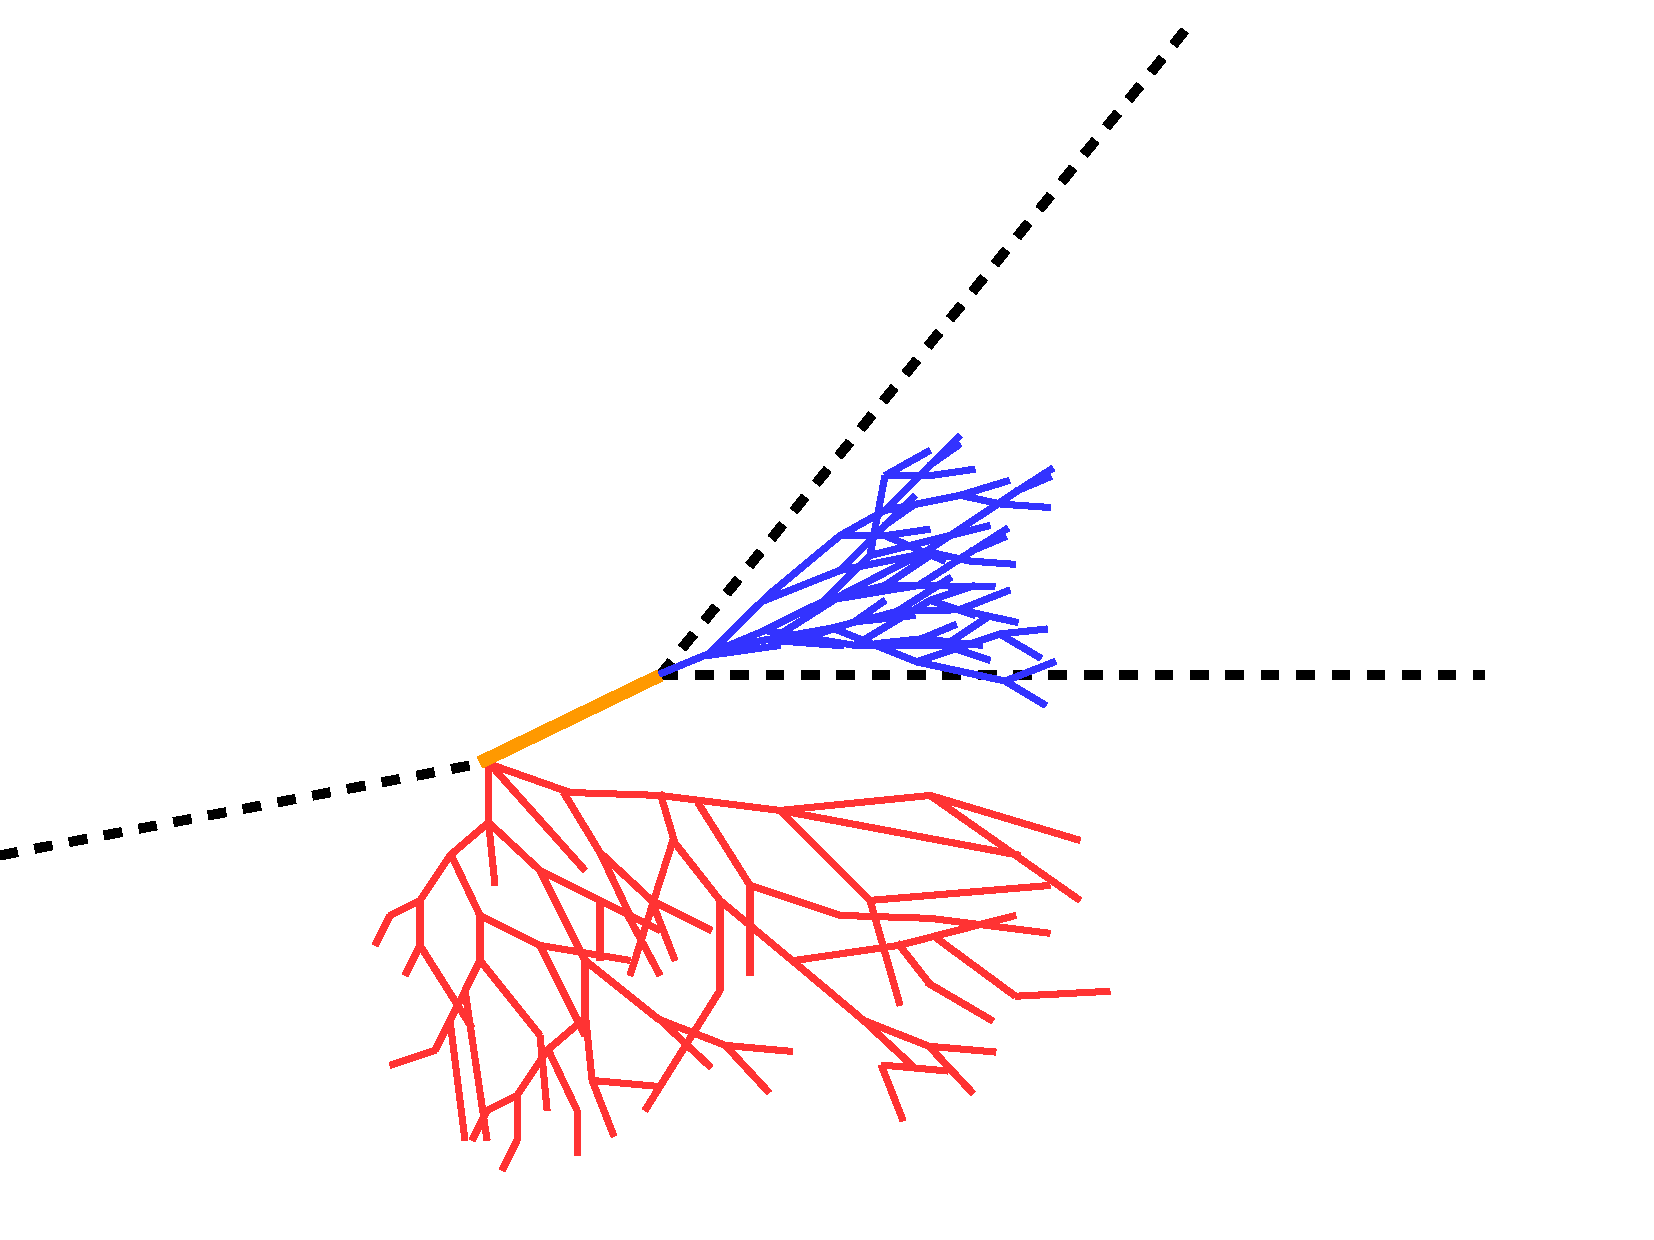
\includegraphics[width=2cm]{figures/neutrinos_properties/interaction_schematics/nutau_CC_cascadeonly.pdf}
            & $\tau^\pm$ decaying into $e^\pm$ or hadrons ($\sim$83\% BR)  
            & \\

            \cmidrule{1-3} CC $\overset{(-)}{\nu_e}$ 
            & 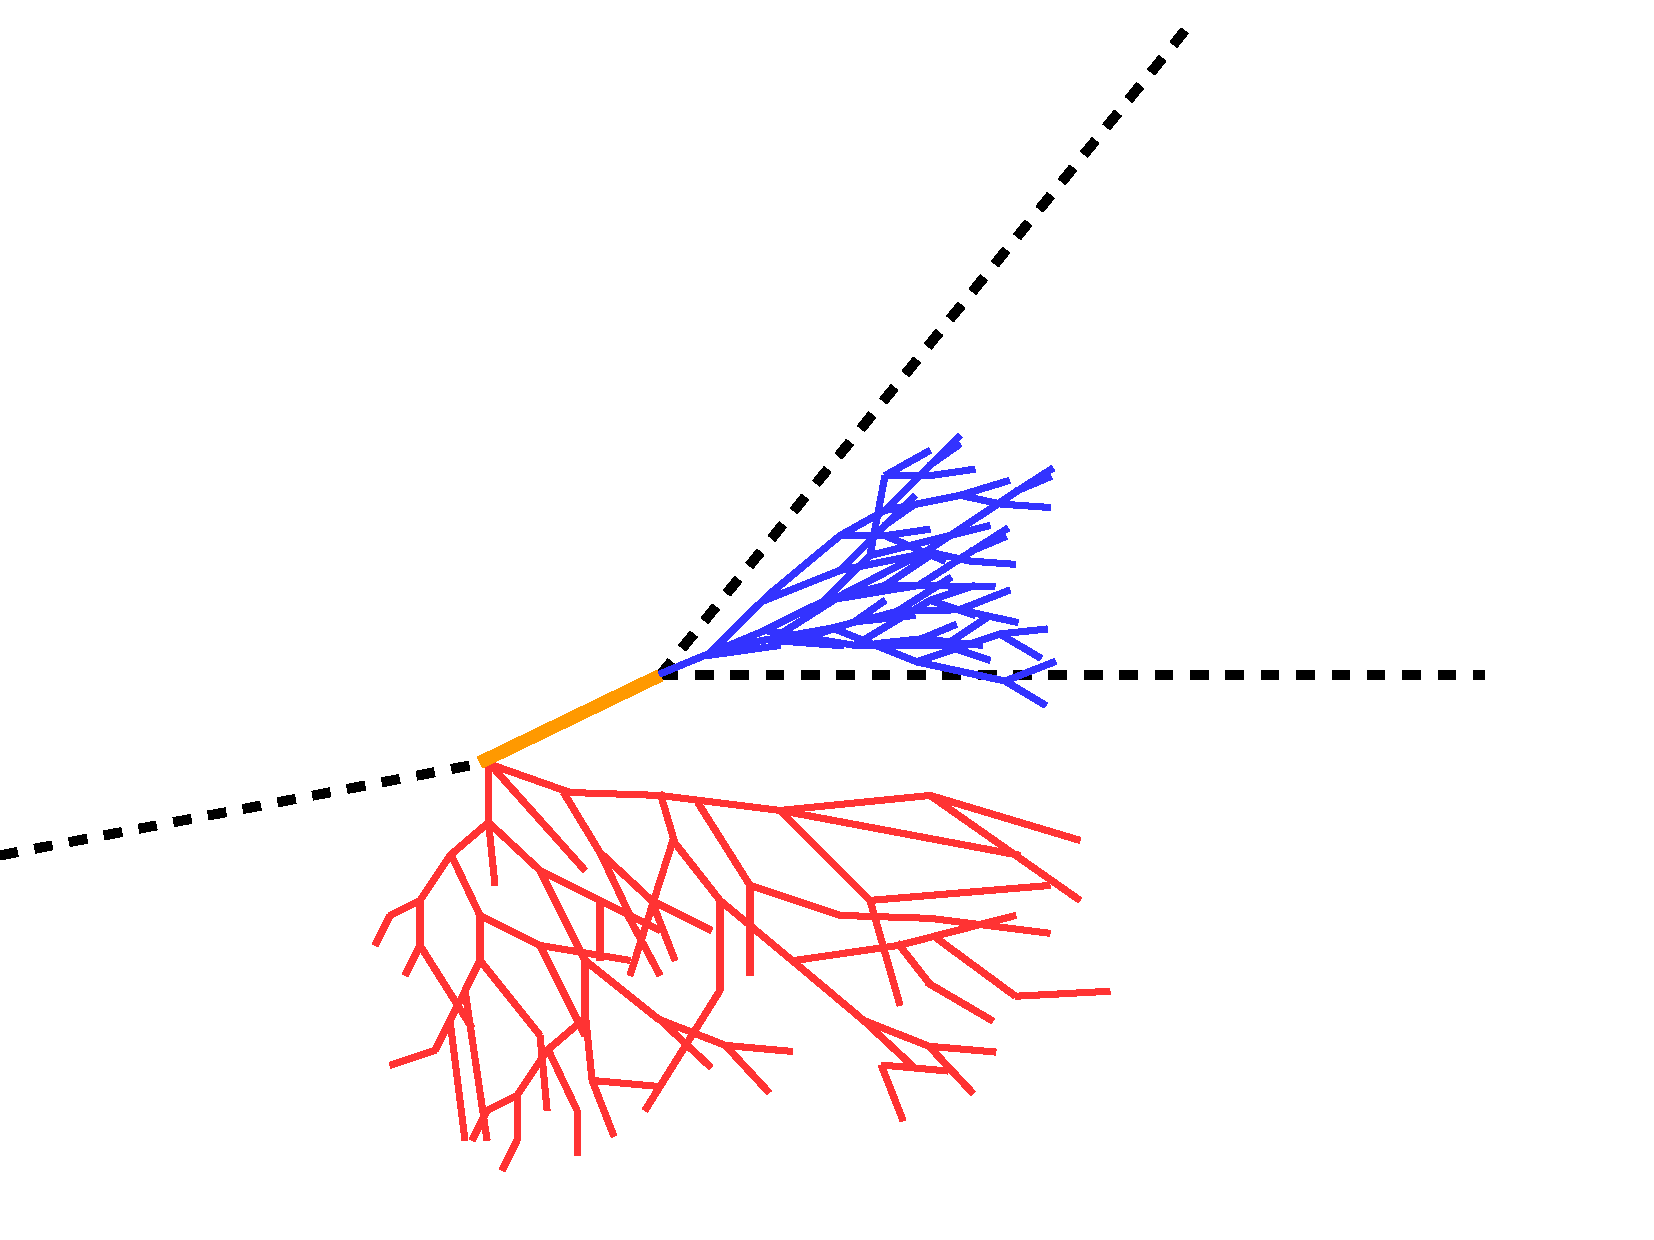
\includegraphics[width=2cm]{figures/neutrinos_properties/interaction_schematics/nue_CC_cascadeonly.pdf}
            & $e^\pm$, hadrons & {Cascade-only} \\

            \cmidrule{1-3}

            NC $\overset{(-)}{\nu_\ell}$ 
            & 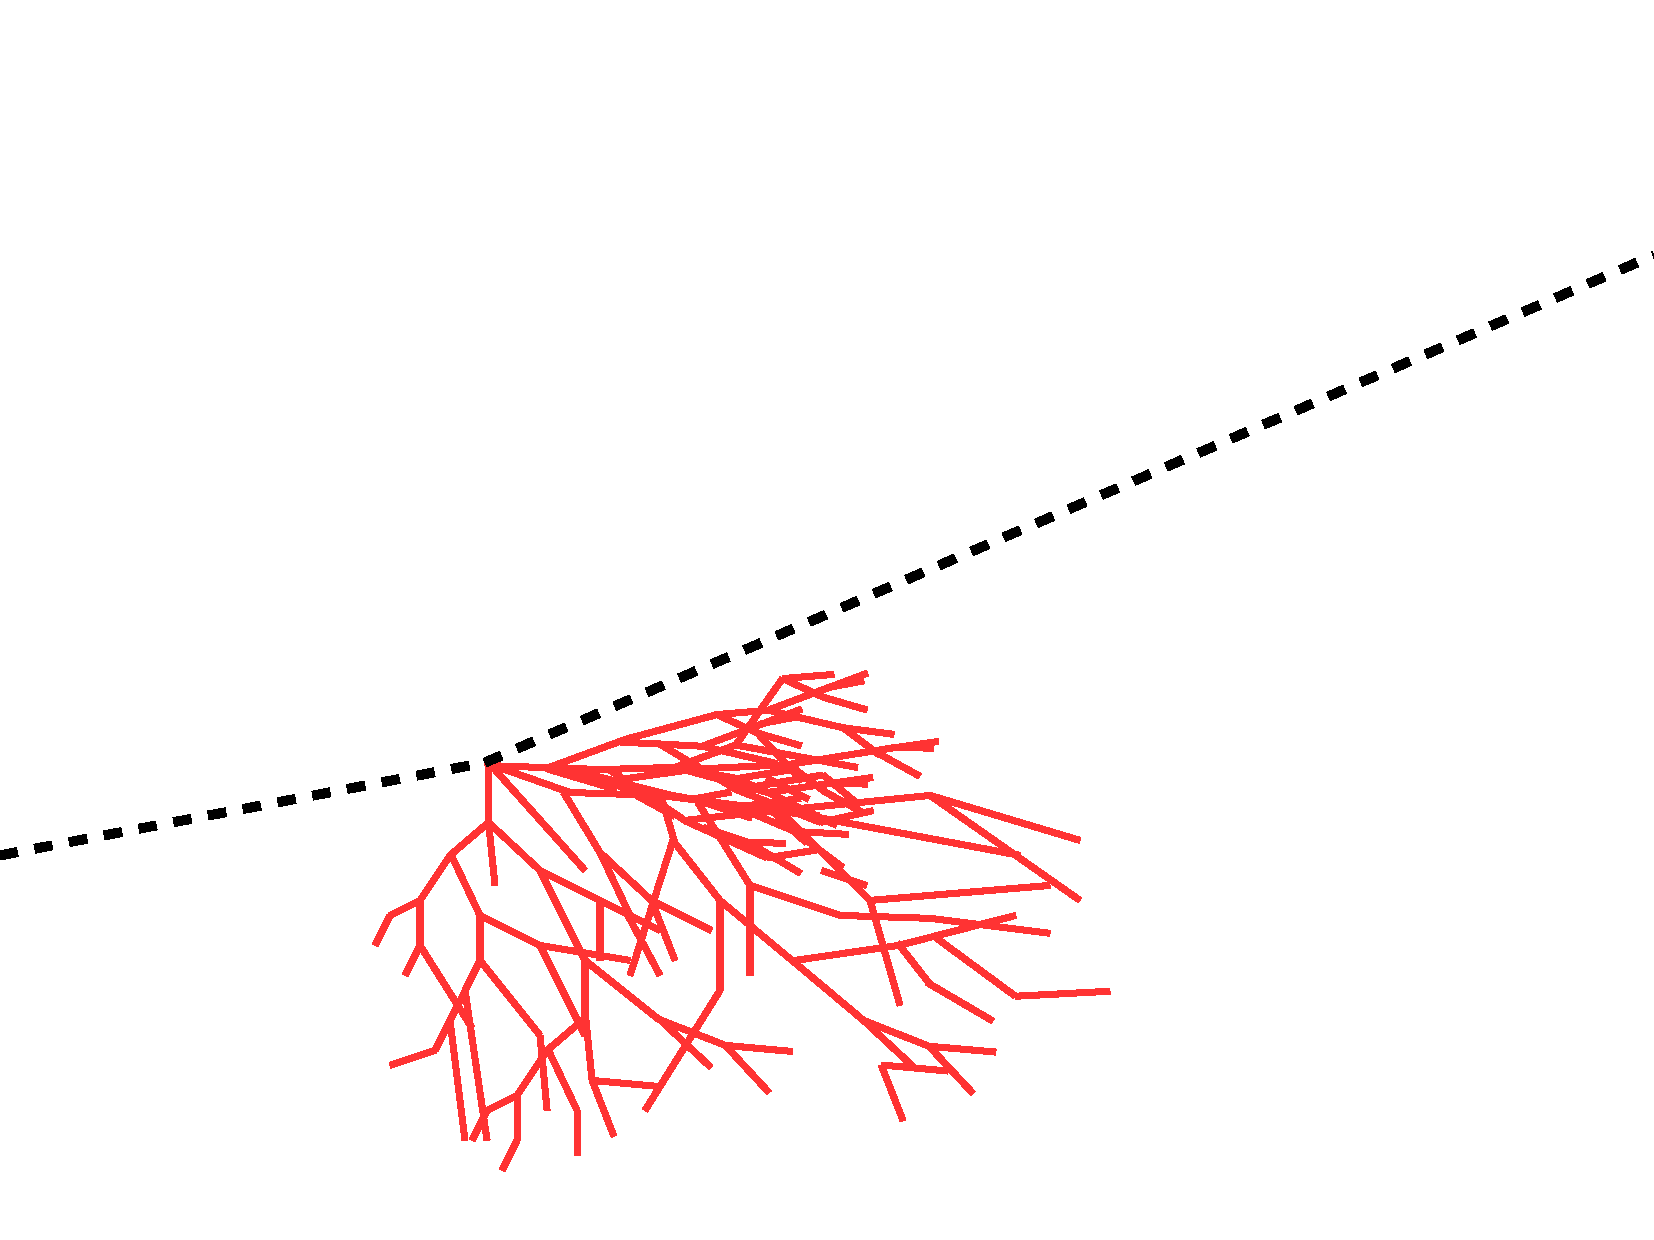
\includegraphics[width=2cm]{figures/neutrinos_properties/interaction_schematics/nuall_NC_cascadeonly.pdf} 
            & hadrons & \\

            \hline
        \end{tabular}
    \end{center}
    \caption[IceCube low energy event signatures and underlying interactions]{IceCube low energy event signatures, their underlying interaction type, and the particles that produce them. Also shown are the secondary particles produced in the interactions. Black dashed lines represent neutrinos, green lines muons, orange line leptons, and blue and red lines are particles in electromagnetic and hadronic cascades, respectively. Adapted from~\cite{ATerliuk}.}
    \labtab{interactions_vs_signatures}
\end{table}


\textbf{Neutrino} interactions are observed as cascades, tracks, or a combination of both, depending on the initial flavor and the interaction type for the specific event.

In $\nu_\mu$-CC interactions, a muon is produced in addition to a hadronic shower. If the interaction happens outside the detector, but the muon passes through the detector, this will create a track-like signature. The same happens if the interaction happens inside, but the energy transfer to the nucleus is small ($y \approx 0$). At energies relevant for this work, tracks have length at the same order of the distance between DOMs, so they can be observed as such.

If the interaction happens inside the detector and the energy transfer to the hadronic part of the shower is larger, it will create a cascade with a track leaving it. A similar signature is observed after a $\nu_\tau$-CC interaction, in which a tau is produced that later decays into a muon, with a branching ratio of $\SI{17}{\percent}$. In those cases the muon usually has a lower energy and the track will be fainter and harder to observe.

The other $\SI{83}{\percent}$ of $\nu_\tau$-CC interactions produce a tau that decays into an electron or hadrons, leaving a cascade-only signature through the electromagnetic or hadronic shower. All $\nu_e$-CC interactions produce pure cascades, since the electron quickly loses its energy in an electromagnetic shower. In all $\nu$ - NC interactions, the produced neutrino escapes and only the hadronic shower is observable. Since the size of the cascades at the energy range of interest is smaller than the spacing of the DOMs, they are approximately observed as point-like, spherical light sources. This is just an approximation, though, and some asymmetry remains in the light profile, which can be used to reconstruct the direction of the incoming neutrino.


\textbf{Atmospheric muons} also produce pure track-like signatures, similar to $\nu_\mu$-CC interactions happening outside the detector. They are one of the main backgrounds for analyses using atmospheric neutrinos and are therefore the target of many filter steps described in \refsec{trigger_and_filter}.
